

\documentclass[conference]{IEEEtran}
\ifCLASSINFOpdf
   \usepackage[pdftex]{graphicx}
\else

\fi
\usepackage[cmex10]{amsmath}
\usepackage{amssymb}
\usepackage{wrapfig}
\usepackage{url}
\usepackage[caption=false,font=footnotesize]{subfig}
\hyphenation{op-tical net-works semi-conduc-tor}
\usepackage{algpseudocode}


\begin{document}


\title{Interactive Online Learning for Obstacle Classification on a Mobile Robot}


\author{\IEEEauthorblockN{Viktor Losing\IEEEauthorrefmark{1}\IEEEauthorrefmark{2},
Barbara Hammer\IEEEauthorrefmark{1} and
Heiko Wersing\IEEEauthorrefmark{2}}
\IEEEauthorblockA{\IEEEauthorrefmark{1}Bielefeld University, Universit\"atsstr. 25, 33615 Bielefeld}
\IEEEauthorblockA{\IEEEauthorrefmark{2}HONDA Research Institute Europe, Carl-Legien-Str. 30, 63073 Offenbach am Main}
}



\maketitle


\begin{abstract}
We present an architecture for incremental online learning in high-dimensional feature spaces and apply it on a mobile robot. 
The model is based on learning vector quantization, approaching the stability-plasticity problem of incremental learning by adaptive insertions
of representative vectors. 
We employ a cost-function-based learning vector quantization approach and introduce a new insertion strategy optimizing a cost-function based on
a subset of samples. 
We demonstrate this model within a real-time application for a mobile robot scenario, where we perform interactive real-time learning of visual categories.
\end{abstract}

\IEEEpeerreviewmaketitle

\section{Introduction}
Incremental learning methods gain a lot of attention nowadays \cite{6628010}, \cite{hoi2014libol}:
highly variable applications 
require flexible algorithms adapting to new trends in the data as well as learning with limited resources from
endless streams. In this situation, classical offline methods are inapplicable due to their dependency on the full data set and necessity for a complete retraining.
The flexible adaptation of technical systems to user habits and preferences is very important for their acceptance,
as noted for the lerning Nest thermostat \cite{Yang:2013:LLT:2493432.2493489}.
Also other fully autonomous devices such as robotic vacuum cleaners or lawn mowers largely benefit from learning 
their application environment and keeping it up-to-date \cite{Forlizzi:2006:SRD:1121241.1121286}. 
Even though a few incremental versions of offline methods have been proposed \cite{1682016}, \cite{conf/iberamia/DiasC08}, \cite{cauwenbergs01incrementaldecremental}, there is still a strong demand
for improved algorithms.\\
In this contribution we investigate a flexible
scheme for interactive learning, a predestined application for incremental algorithms \cite{export:238110}.
An online recognition architecture that is capable of interactive learning of up to 50 objects in short time was presented in \cite{PN0805}.
Here we will rely on a similar architecture but incorporate and investigate a richer online learning model.
Vision based incremental learning on a mobile robot was also performed in \cite{4398986}, \cite{4650681}. However, these systems
perform indoors and use different algorithms such as incremental SVM or bag of words.
We demonstrate our framework within a real-time learning scenario which focuses on the challenging task of outdoor object classification on a mobile robot. 
Specific contributions are: 
\begin{itemize}
\item 
Extension of prototype based learning to online scenarios with adjustable model complexity.
\item
Extensive evaluation of different strategies to insert prototypes for these adjusted models.
\item
Integration of this framework into an easy-to-use online learning system paired with a live-labeling app.
\end{itemize}
Prototype-based approaches such as neural gas \cite{martinetz:gas} or learning vector quantization (LVQ) \cite{kohonen-self-organizing-maps-2001} are popular options among 
online learning algorithms, with applications ranging from biomedical data analysis \cite{10.1371/journal.pone.0059401}, image recognition \cite{journals/neco/WersingK03}, 
to robotics \cite{Carlevarino00anincremental}. Due to their successful application we will focus on such models, in particular supervised LVQ.\\
The ability of structure adaptation according to the complexity of a given task is helpful and becomes even more crucial with regards to big or streaming data sets violating the assumption of data being i.\,i.\,d.\,\cite{Carlevarino00anincremental}, \cite{6853440}.
Dynamic prototype insertions and deletions enable this flexibility intuitively. Moreover, these can be done in an efficient and incremental way since they affect the model only locally. \\
Several proposals for placement strategies of prototype insertion, based on heuristics,  were made  in \cite{DBLP:conf/ijcnn/GrbovicV09}, \cite{DBLP:conf/esann/BermejoCP98}, \cite{PN0805}.
In contrast, our proposal relies on the derivation of LVQ
 as cost function optimization;
it optimizes an approximation of these costs for improved robustness. 
Since we confine the optimization on a limited number of recent samples, the resulting
implementation offers the advantages of an adjustable and strictly
limited memory consumption paired with linear complexity.
Such linear time and constant memory conditions are
especially relevant for efficient mobile applications. 

\section{Generalized LVQ}\label{relatedWork}
\newcommand{\x}{\mathbf{x}}
\newcommand{\w}{\mathbf{w}}
Given a classification task of $C$ classes, the training set $X= \{ (\mathbf{x}_i,y_i) \in \mathbb{R}^n \times \{1,...,C\}\}_{i=1}^m$ is approximated
by an LVQ classifier with a set of $p$ prototypes $W= \{(\mathbf{w}_j,l_j) \in \mathbb{R}^n \times \{1,...,C\}\}_{j=1}^p$.
The Voronoi region of a prototype $(\w_j,l_j)$ is defined as 
$V_j=\{\mathbf{x} \in X|$ $\Vert \mathbf{x}-\mathbf{w}_j\Vert \leq \Vert \mathbf{x}-\mathbf{w}_k\Vert \ \forall \ j \neq k\}$.
A given data point $\x_i$ is classified according to the label of its closest prototype using a distance measure $d$ such as the squared Euclidean distance $d(\x,\w) = \Vert\x-\w\Vert^2$.\\
Sato and Yamada introduced the generalized LVQ (GLVQ) \cite{conf/nips/SatoY95} which, in contrast to previous heuristic approaches, minimizes the cost-function
\begin{equation}\label{eq:costFunction}
E(X,W)=\sum_{i=1}^{m} \Phi((d^+_i-d^-_i)/(d^+_i+d^-_i)),
\end{equation}
where $\Phi$ is a monotonically increasing function, e.\,g.\ the logistic function. The distance of a sample $\x_i$ to its closest prototype $\w^\pm$ of the correct / incorrect class is
denoted by $d^{\pm}_i$.
By updating the prototypes for each data point as follows
\begin{equation}\label{eq:glvqUpdate}
\w^\pm := \w^\pm-\lambda \frac{\partial E(X,W)}{\partial \w^\pm},
\end{equation} 
where $\lambda$ is the learning rate, the cost function is minimized in a stochastic gradient descent scheme.

\section{Learning Architecture}\label{IncrementaLearningMethod}
\iffalse
\begin{figure}
\begin{algorithmic}
  \Function{Learn}{$\Psi$, $\hat{t}$, $(x,y)$, $errCount$, $errThresh$}
  \State $get\ prototypes\ w^\pm\ and\ distances\ d^\pm\ to\ (x,y)$
  \State $add\ (x,y),\ d^\pm\ to\ \Psi$
  \State $update\ w^\pm\ according\ to\ \eqref{eq:glvqUpdate}$
  \State $decrease\ learning\ rate\ of\ w^\pm$
  \If{$d^- < d^+$}
    \State $errCount := errCount + 1$
    \If{$errCount \geq errThresh$}
      \State $insert\ new\ prototype\ using\ \Psi,\ \hat{t}$
      \State $errCount := 0$
    \EndIf
  \EndIf
  \EndFunction
\end{algorithmic}
\caption{Pseudo code for the placement strategy SamplingCost} 
\label{fig:learning}
\end{figure}
\fi

We solely focus on supervised learning from data-streams. Every prototype $\w_j$ has its own linearly decreasing learning rate $\lambda_j$ to approach the stability-plasticity dilemma \cite{PN0805}.
As an overview, the learning architecture works as follows:\\
The learning architecture initially does not have any prototype, i.\,e.\ $W=\emptyset$.
For each new sample $(x_i,y_i)$ we test whether $y_i$ is a new class.
If $y_i$ is not yet represented in the model, this sample is directly added as a prototype.
Otherwise, we
perform the GLVQ-updates \eqref{eq:glvqUpdate} and store the sample with its distance information in a short term memory of limited size, replacing old ones if necessary. 
If the sample is misclassified we increment an error count. As soon as a predefined number of errors occurs, the employed placement strategy provides a new prototype which 
is added to the set of prototypes $W$. Then, we update distances within the short term memory.
The error count is reset and we start over again.
In the remainder of the section, the single steps are described in more detail. 
\subsection{Limited Sample Memory}\
Apart from the prototypes, we maintain a short term memory which is defined as a list
\begin{equation}\label{eq:Psi}
\Psi:= [ (\x_i,y_i,d^+_i,d^-_i) \ |\ i \in \{1,...,t\}],
\end{equation}
containing entries for the recent $t$ samples. Every additional sample leads to the deletion of the oldest entry as soon as the limit of $t$ stored entries is reached,
i.\,e.\ $|\Psi|=t$. Therefore, the memory consumption of the system is limited, which is crucial for online learning. 
Based upon $\Psi$, placement strategies propose new prototypes.\\
The GLVQ-updates \eqref{eq:glvqUpdate} change prototype positions and corresponding sample distances.  
However, we neglect these changes within$\Psi$ for the sake of efficiency. 
Hence $\Psi$ contains approximations of the actual distances and their quality depends on the magnitude of 
the learning rates $\lambda_j$ as well as on the window size $t$. During our experiments, this simplification had negligible 
or even no consequence on the systems' performance. We used a window size of $t=200$ for all experiments.

\subsection{Insertion Timing}
Insertion timing is based on error counting as already proposed in \cite{PN0805}.
Whenever the error count reaches a threshold, a new prototype is added and the error count is reset to zero. 
This simple and computationally cheap approach couples growing speed strictly with systems' performance on training data. 
The learning architecture evolves fast in case of low accuracy but changes
only slightly when few errors are made. Consequently, a system will grow as long as it does not classify perfectly (i.e.\ infinitely in case of overlapping classes). 
%In case of overlapping 
%distributions, the growth is unlimited. 
This could easily be avoided by a restriction of
the incremental growth to cases which significantly improve
the GLVQ cost function. However, this
goes beyond the scope of this paper.

\subsection{Insertion of Prototypes}
Whenever a new prototype $(\w,l)$ is proposed by a placement strategy and inserted into the network, i.\,e.\ ${W}:= W \cup (\mathbf{w},l)$, $\Psi$ is updated in the following way:\\
\begin{equation}\label{eq:PSIUpdate}
\begin{align*}
&\forall\ (\mathbf{x}_i,y_i,d^+_i,d^-_i)  \in \Psi: \\
&\ \ \ d^+_i := d(\x_i,\w), \ \mathrm{if}\ y_i=l \land d^+_i > d(\x_i,\w)\\
&\ \ \ d^-_i := d(\x_i,\w), \ \mathrm{if}\ y_i\neq l \land d^-_i > d(\x_i,\w).
\end{align*}
\end{equation}

\subsection{State of the Art Placement Strategies}\label{placementAlgorithms}
Each placement strategy proposes one new prototype whenever a predefined number of errors is reached.\\
We compare our proposal with three other strategies from the literature, which solely rely on misclassified samples. The set of misclassifications can be easily  extracted
from $\Psi$ as $\Upsilon=\{ (\x_i,y_i)\ |\ (\x_i,y_i,d^+_i,d^-_i) \in \Psi \land d^+_i > d^-_i\}$. 
The strategies select one prototype based on $\Upsilon$ as follows:\\
\textit{a) Closest:}
In \cite{PN0805} Kirstein et al.\ propose to select those misclassified samples as candidates that are the closest to prototypes of another class. 
This choice shall lead to insertions along class borders. Candidates are ordered ascendingly by their distance to the nearest wrong class.\\ 
\textit{b) Cluster:}
Grbovic et al.\ cluster misclassified samples per class and select centroids of the biggest clusters as new prototypes \cite{DBLP:conf/ijcnn/GrbovicV09}.
Therefore, the cluster-size is the ranking criterion for candidates. We used k-Means to cluster misclassifications. Since $k$ has to be predefined, 
the common rule of thumb $k=\sqrt{\frac{n}{2}}$ was utilized. However, this value was multiplied by a factor of two to achieve the best experimental results.
\textit{c) Voronoi:}
A similar approach was chosen by Bermejo \cite{DBLP:conf/esann/BermejoCP98}. But instead of clustering, he determines the Voronoi region containing the most misclassified samples of one class. 
The mean of these samples is chosen as a new prototype.
\setcounter{figure}{0}

\subsection{Proposed Placement Strategy: SamplingCost}
The proposed new strategy relies on an optimization of the GLVQ-cost-function which is approximated by
the sample $\Psi$. Thereby, prototypes are taken from candidate positions
from a random subset $\hat{\Psi}\subseteq \Psi$ of size $|\hat{\Psi}|=\hat{t}$ only.
For every candidate $(x_i,y_i)$ in $\hat{\Psi}$,
its effect on the costs can efficiently be approximated as follows:
\begin{itemize}
\item[1.] 
Extend $\hat{W}:= \{W\cup (x_i,y_i)\ \}$.
\item[2.]
Update ${\Psi}$ as described in \eqref{eq:PSIUpdate} but store the result temporarily in another list ${\Psi'}$.
\item[3.]
Calculate the cost-function value $E(\Psi', \hat{W})$ on the basis of the distances stored in $\Psi'$. 
\end{itemize}
The sample with smallest value $E(\Psi', \hat{W})$  is added as a new prototype to $W$,
and $\Psi$ updated accordingly. The complexity is ${\cal O}(\hat{t}\cdot t)$ and pseudo code is depicted in Figure \ref{fig:SamplingCost}.
\begin{figure}
\begin{algorithmic}
  \Function{SamplingCost}{$\Psi$, $\hat{t}$}
  \State $minCost := 1$
  \State $proto := null$
  \State $\hat{\Psi} := getRandomSubset(\Psi, \hat{t}$)  
  \ForAll {$(x,y) \in \hat{\Psi}$}
    \State ${\Psi'} := updateShortTermMemory(\Psi, (x,y))$
    \State $cost := calculateCost(\Psi')$
    \If{$cost < minCost$}
      \State $minCost := cost$
      \State $proto := (x,y)$
    \EndIf
  \EndFor
  \State \Return $proto$
  \EndFunction
\end{algorithmic}
\caption{Pseudo code for the placement strategy SamplingCost} 
\label{fig:SamplingCost}
\end{figure}

\section{Artificial Data}
We compare these different placement strategies by integrating each approach separately in
an online learning architecture. 
The resulting four online learning algorithms are trained using identical conditions
on two artificial data sets with different characteristics. 
The main aim of these two-dimensional data sets is to investigate how precisely the strategies can represent the real class borders.
The arrangement of these problems is shown in Figure \ref{Borders}.  
\begin{figure}
\centering
	\subfloat{%
	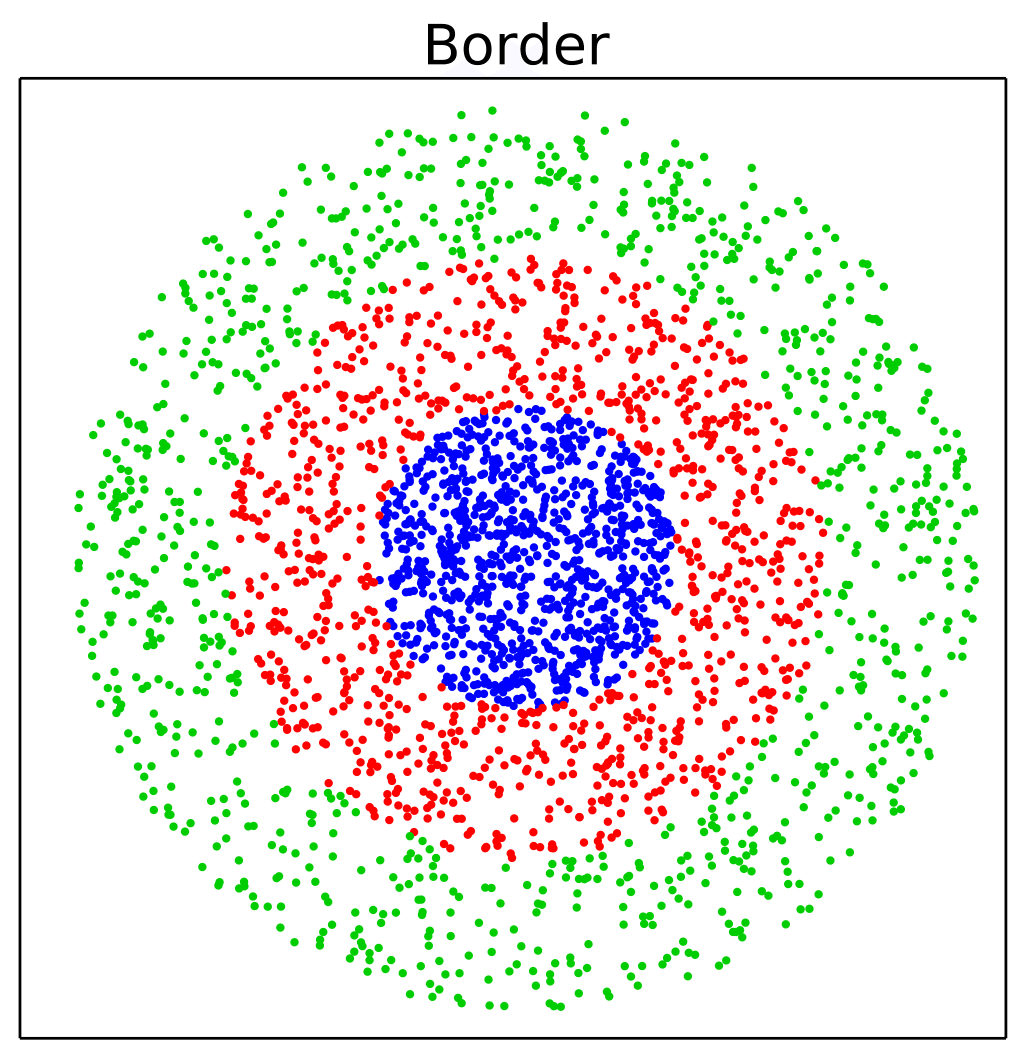
\includegraphics[width=0.15\textwidth]{Images/Toy/Border_random_07_0_initial.png}
	}
	\subfloat{%
	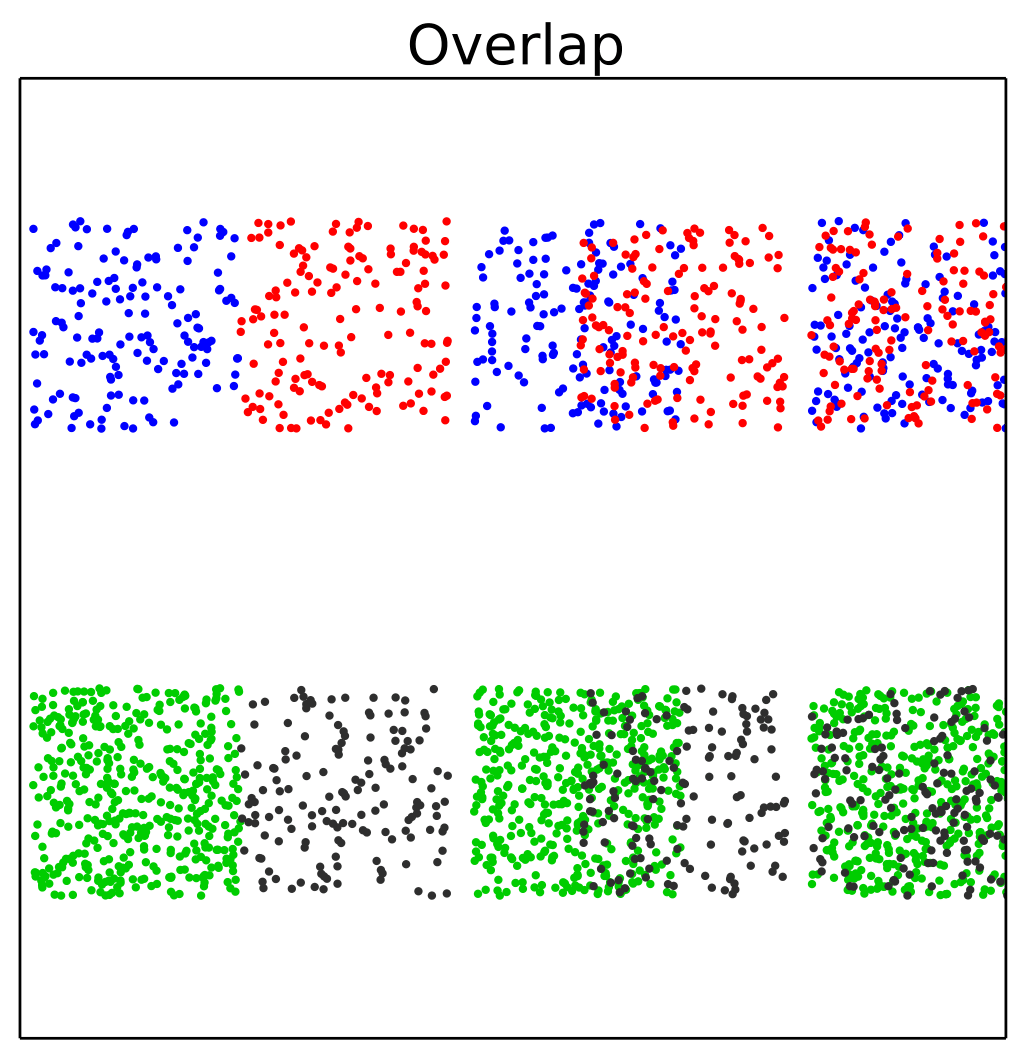
\includegraphics[width=0.15\textwidth]{Images/Toy/Overlap_random_07_0_initial.png}
	}	
\caption{Artificial data sets \textit{Border} and \textit{Overlap}. Different classes are coded by different colors. 
The \textit{Border} data set (Fig.~\ref{Borders}, left) consists of three circular classes. Each class consists
of 1000 uniformly distributed points.
The data set \textit{Overlap} (Fig.~\ref{Borders}, right) contains uniform squared distributions which overlap to various degrees. The upper row classes have the same densities whereas, below,
the green class is three times denser than the black.}
\label{Borders}
\end{figure}
We used $70\%$ of the data for training and the rest for testing.\\
Overlapping distributions are usually the most difficult to deal with since a complete separation is not possible.
Given an overlap, the densest class should be preferred in the Bayesian optimum. These challenges are incorporated in the \textit{Overlap} data set, visualized in Figure \ref{Borders} on the right.\\
One example of a final prototype arrangement of each strategy can be seen in Figure \ref{fig:Toy1Nets}.
\begin{figure}
        \centering
	\subfloat{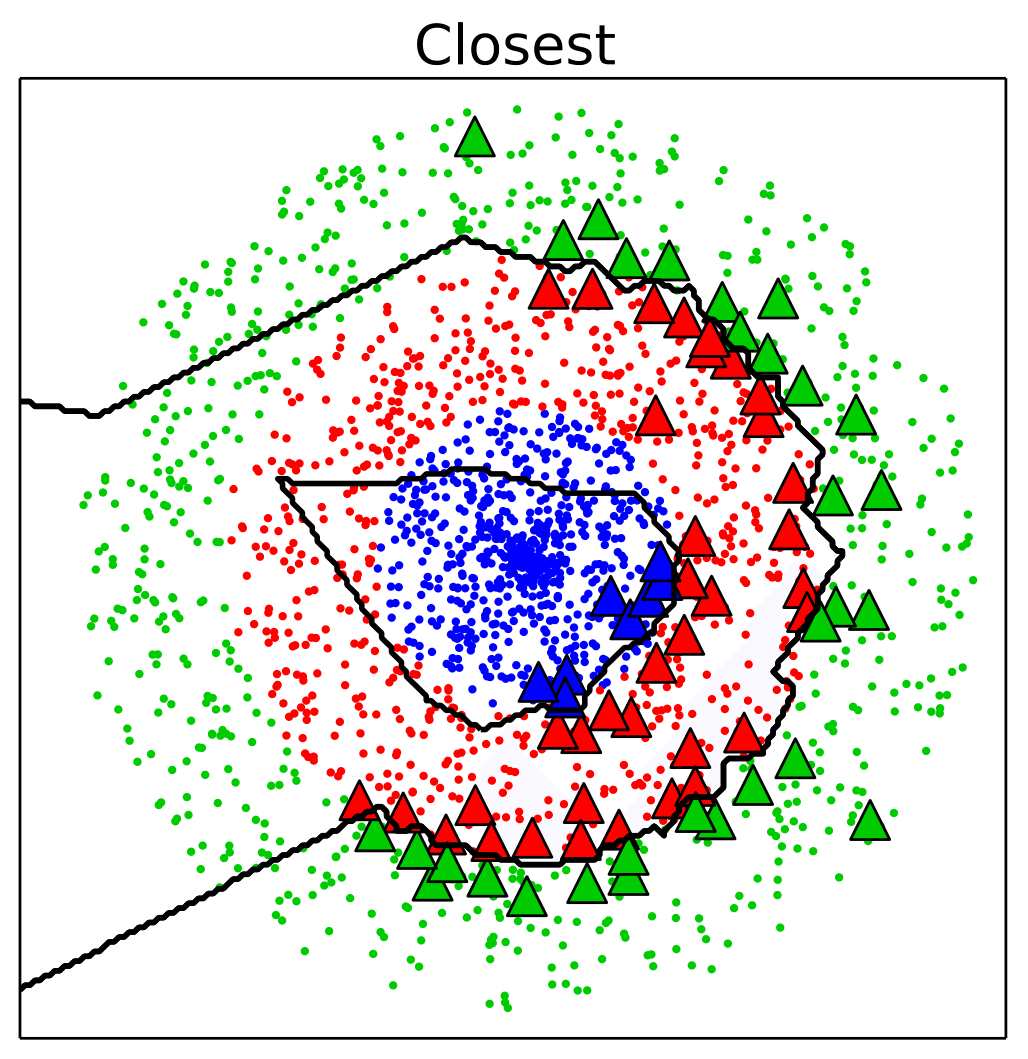
\includegraphics[width=0.12\textwidth]{Images/Toy/Toy1_random_07_Closest_2_final.png}}
	\subfloat{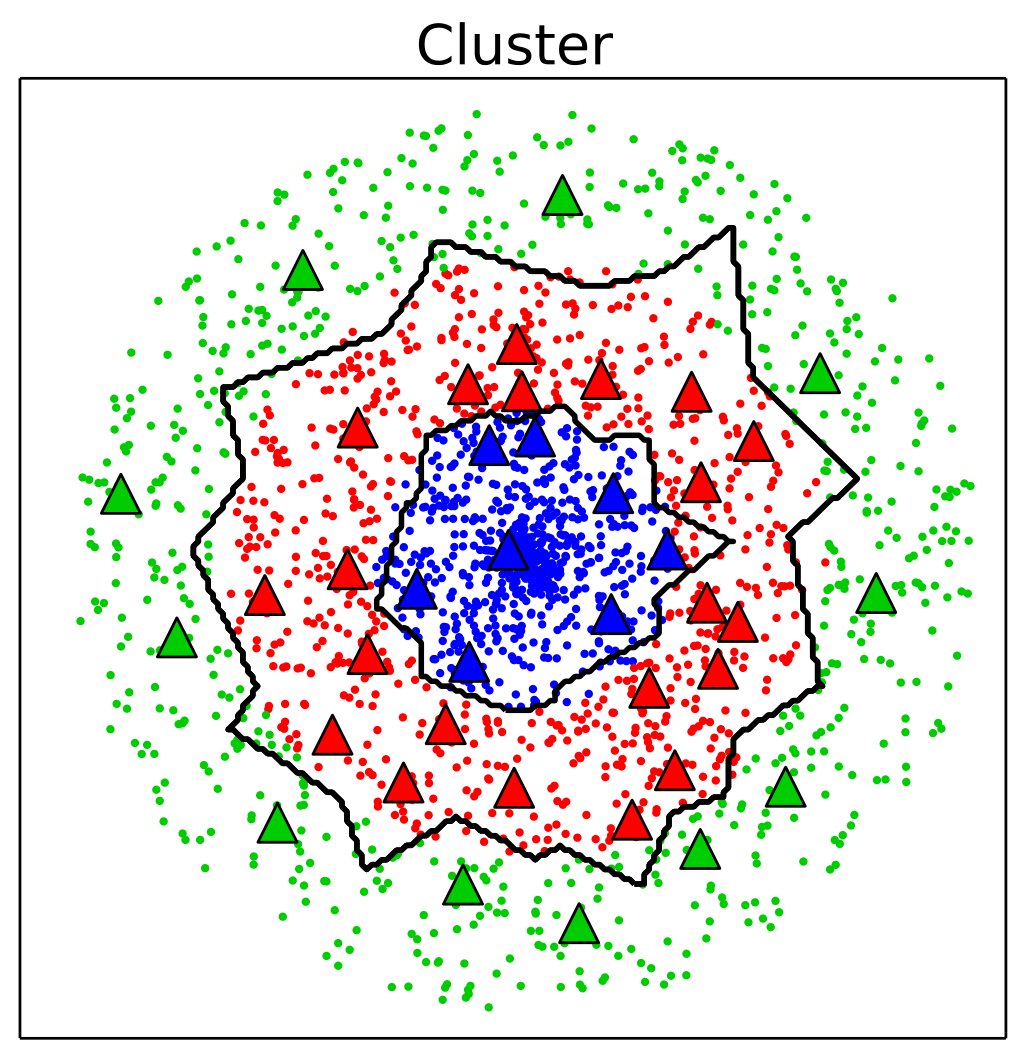
\includegraphics[width=0.12\textwidth]{Images/Toy/Toy1_random_07_Cluster_1_final.png}}
	\subfloat{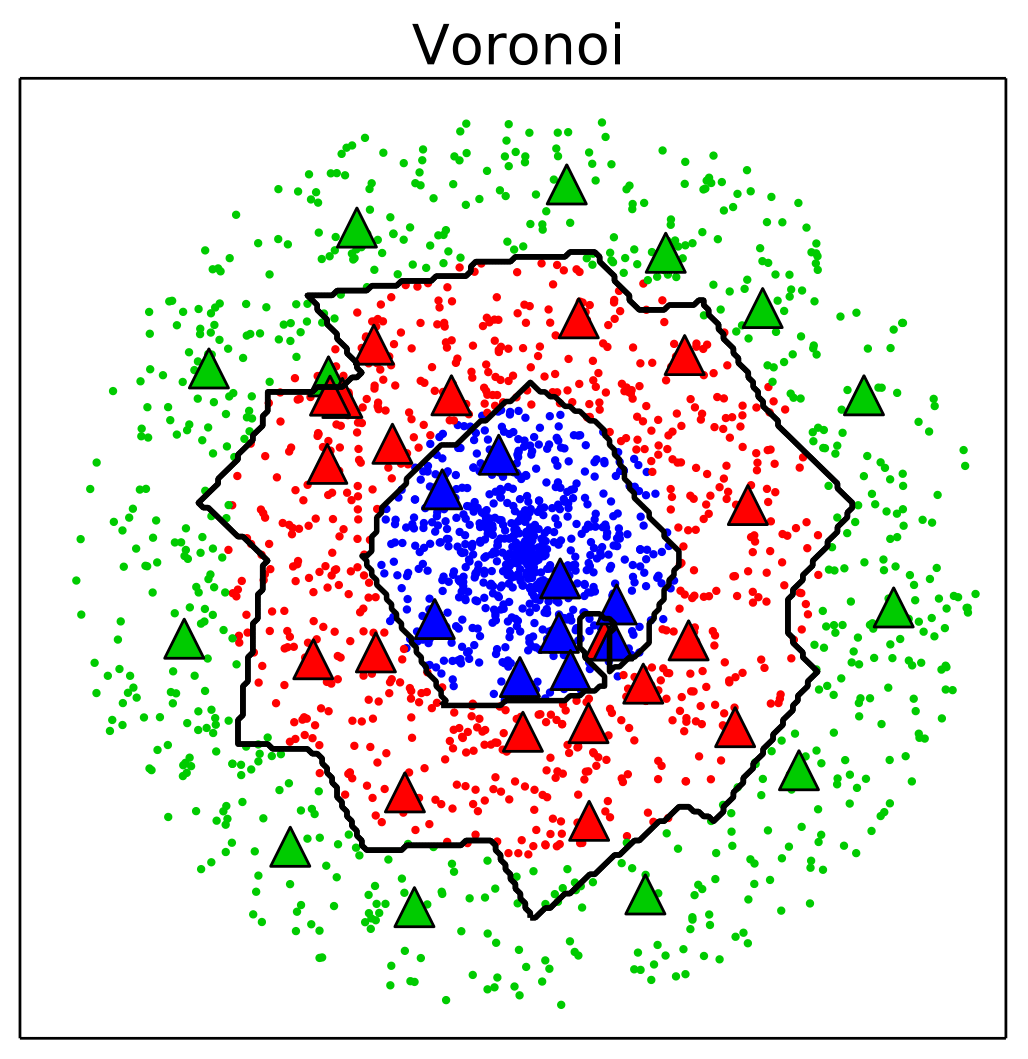
\includegraphics[width=0.12\textwidth]{Images/Toy/Toy1_random_07_Voronoi_0_final.png}}
	\subfloat{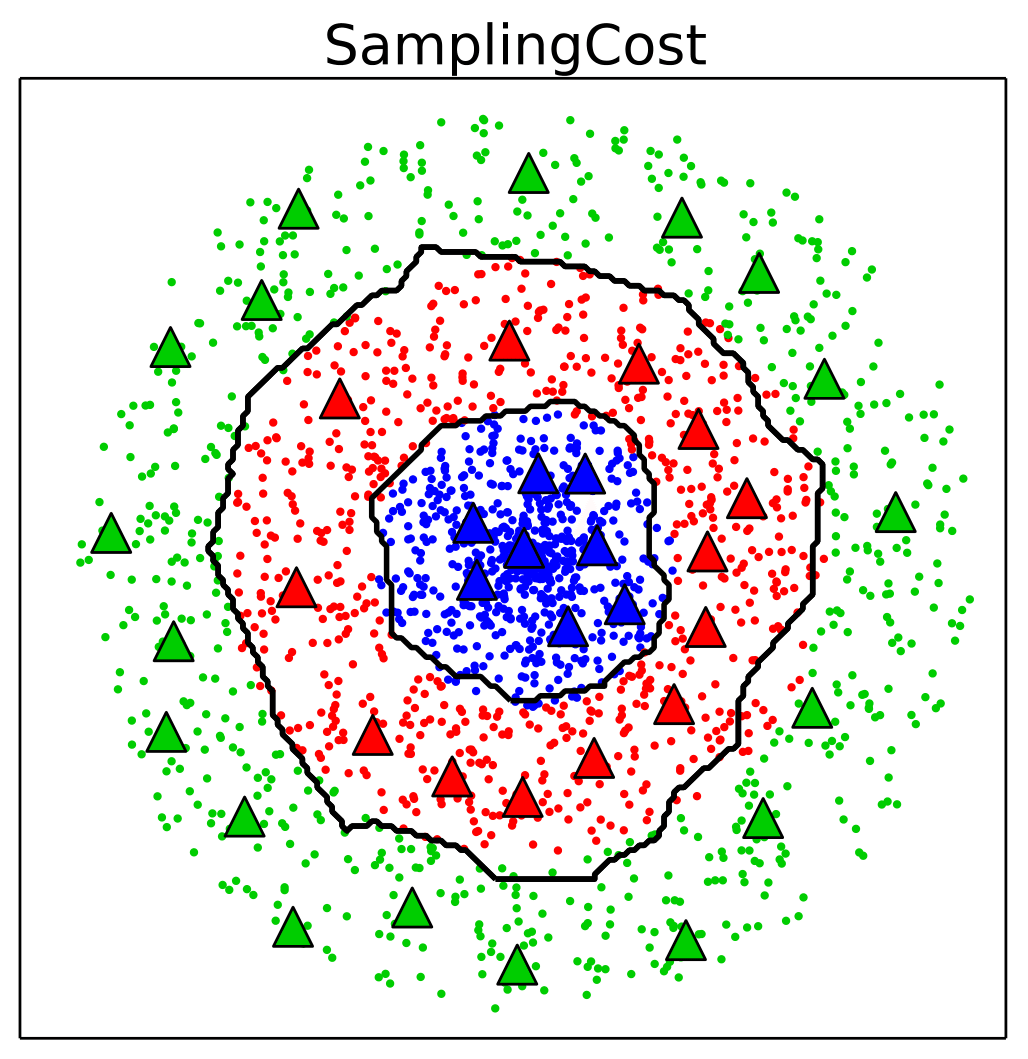
\includegraphics[width=0.12\textwidth]{Images/Toy/Toy1_random_07_SamplingCost_2_final.png}}
	\vspace{0 pt}
	\subfloat{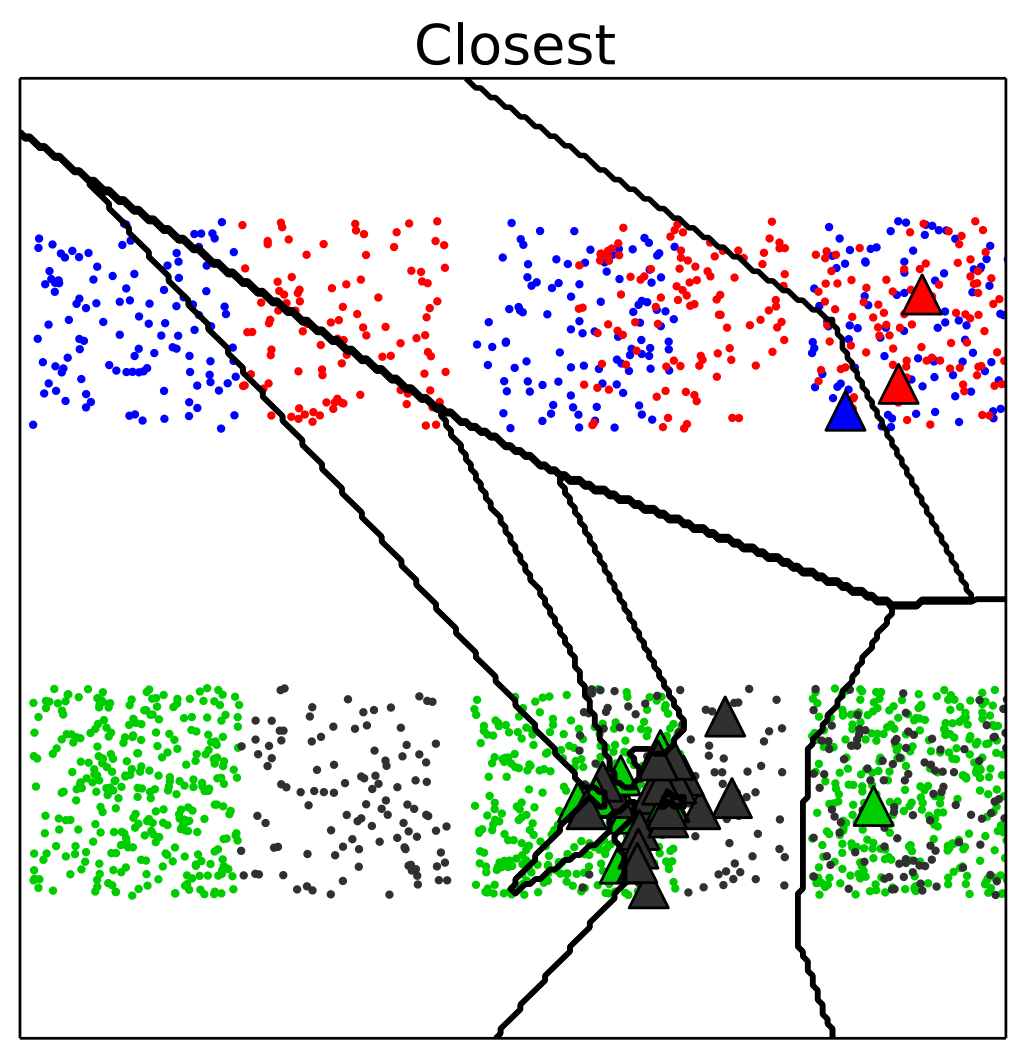
\includegraphics[width=0.12\textwidth]{Images/Toy/Toy3_random_07_Closest_2_final.png}}
	\subfloat{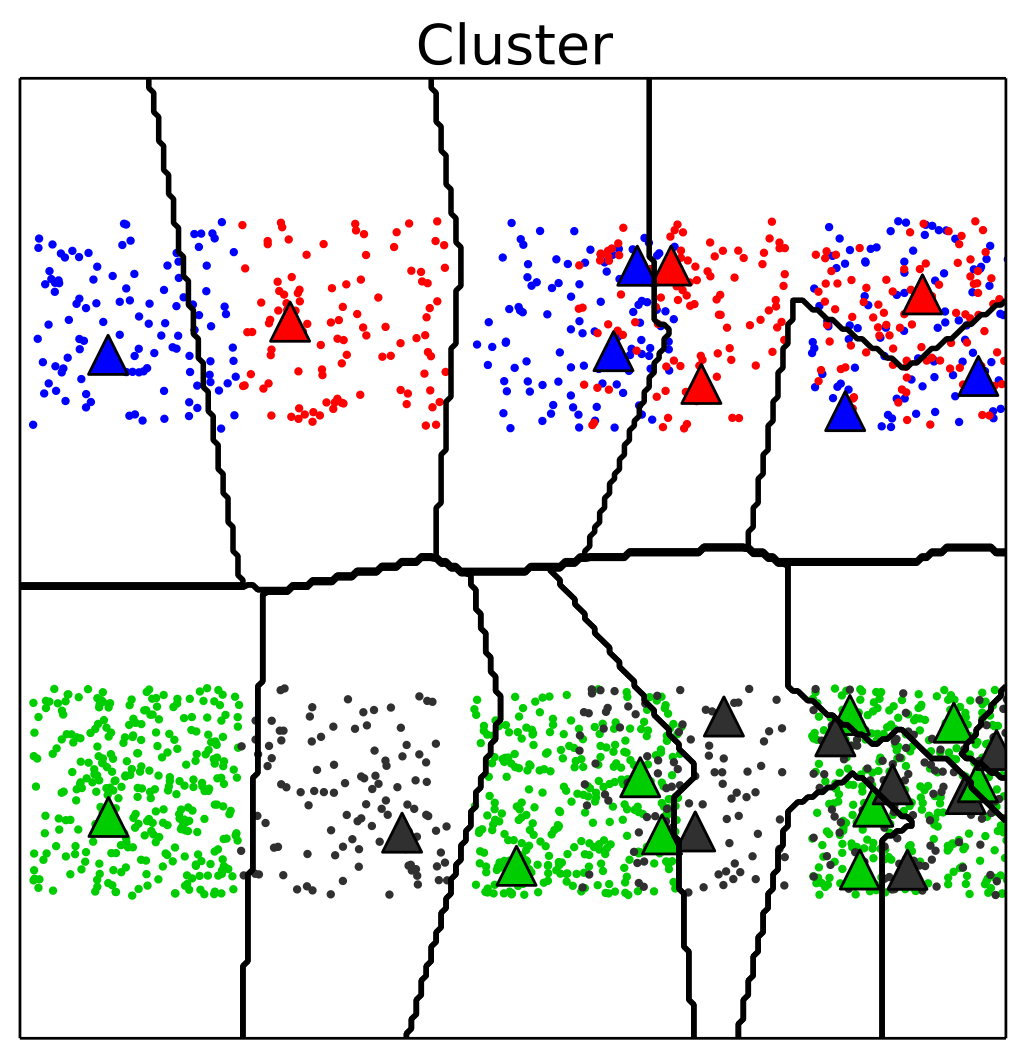
\includegraphics[width=0.12\textwidth]{Images/Toy/Toy3_random_07_Cluster_2_final.png}}
	\subfloat{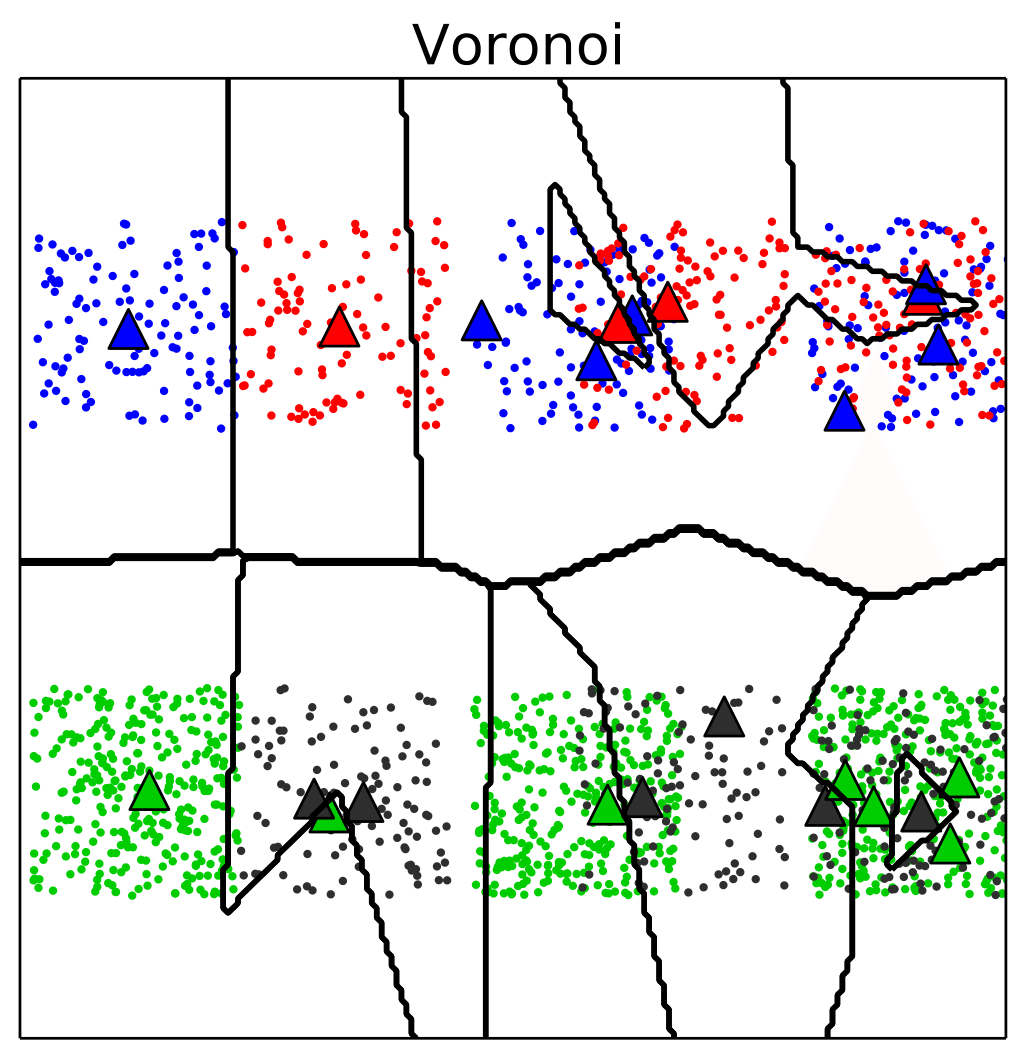
\includegraphics[width=0.12\textwidth]{Images/Toy/Toy3_random_07_Voronoi_2_final.png}}
	\subfloat{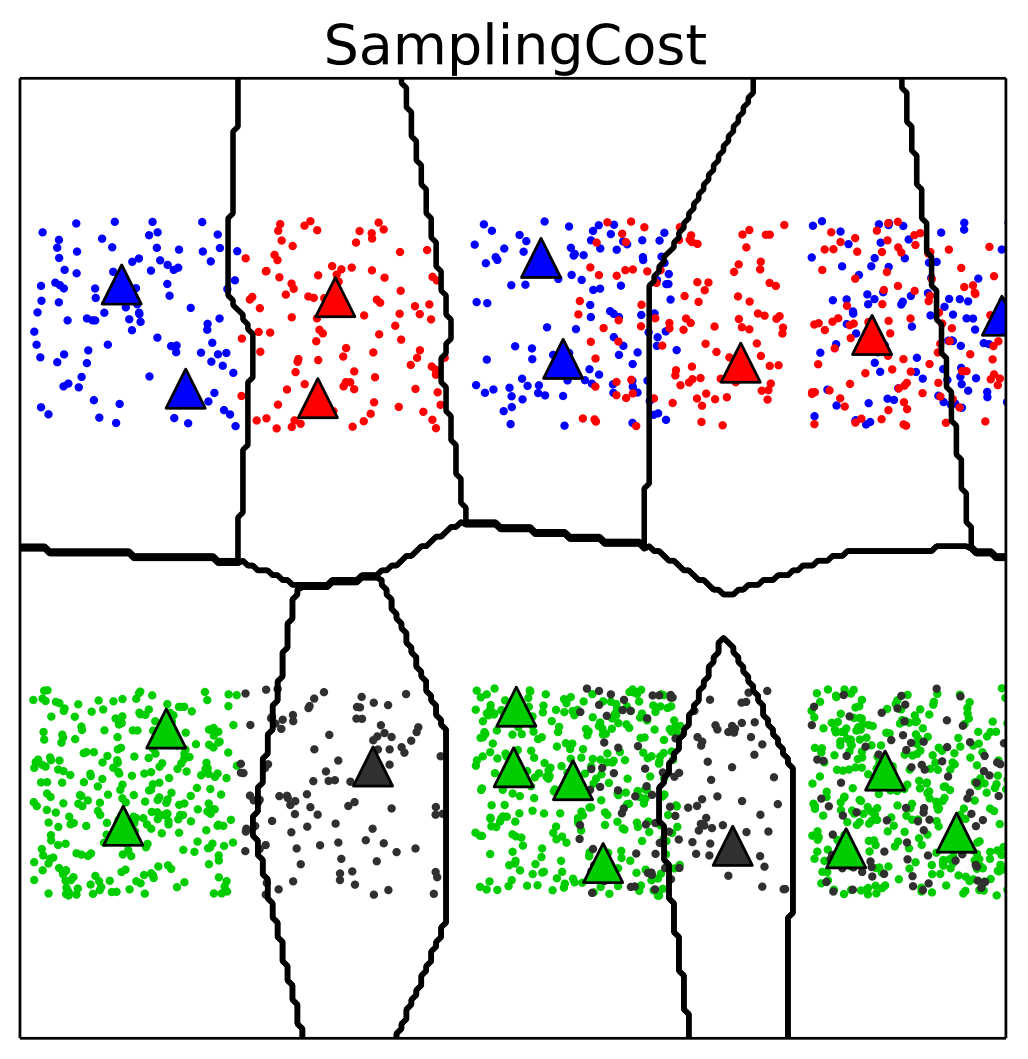
\includegraphics[width=0.12\textwidth]{Images/Toy/Toy3_random_07_SamplingCost_9_final.png}}
        \caption{Networks of each placement algorithm after the training of the data sets \textit{Border} (top) and \textit{Overlap} (bottom). 
        Prototypes are symbolized by triangles and black lines represent the learned class boundaries.}
        \label{fig:Toy1Nets}
\end{figure}
Boundaries generated by \textit{Closest} deviate the most from actual borderlines.
On the \textit{Border} data set, samples are separated very accurately at few specific spots, 
which are clustered with multiple prototypes, but a significant portion of the actual border is uncovered and causes the majority
of misclassifications. Whether a sample is promoted to a prototype or not is solely based on its distance to nodes of other classes. This leads to insertions along 
class borders and explains why the algorithm often gets stuck. A prototype inserted close to a border is very likely to cause new misclassified samples
which are, in turn, closely located to this new prototype. Therefore, many unnecessary insertions
are used to represent class boundaries at specific areas in contrast to some completely neglected parts.
In case of the \textit{Overlap} data set, this problem is even more severe and entraps the algorithm to insert prototypes in one exclusive 
area. \textit{Closest} is very sensitive to noise since a single sample can cause multiple and consecutive prototype insertions.\\
Results of \textit{Cluster} and \textit{Voronoi} look quite similar. Prototypes are spread fairly regular and approximate the actual boundaries well.
In case of ambiguous regions, unnecessary prototypes of both classes are placed regardless whether density proportions between classes are existing or not.
Initially, classes with higher densities are favored because big clusters are likely to be found among them. 
But, as soon as they are covered, prototypes for less dense classes are inserted too and deteriorate the accuracy again.
These strategies perform similarly because both compute clusters of misclassified samples and place prototypes in their centroids. 
The clustering quality is crucial for the performance, since too fine clustering leads to more prototypes than necessary
and too coarse clustering can cause severe misplacement because centroids of too large cluster might be located within samples of another class.
\textit{Voronoi} clusters spatially by incorporating the available Voronoi cells which are shrinking continuously as more nodes are introduced into the net.
Therefore, clustering is coarse initially and fine at the end. The few misplaced prototypes (Fig.~\ref{fig:Toy1Nets}) are caused by the initial coarse clustering.
\textit{Cluster}, on the other hand, utilizes k-Means, which requires the number of clusters as parameter in advance. 
Since a rather high number is chosen, coarse clustering is avoided and the number of samples per cluster is still 
high enough to prevent too fine clustering. Both algorithms are robust against noise because a high amount of accumulated noisy points of the same class 
is necessary to cause an insertion there. \\
\textit{SamplingCost} reproduces the true class borders the most accurately. It distributes nodes regularly over the samples and
 balances the tradeoff between prototypes being placed as close as possible to samples of its own class and far from those of another class.
Its cost-function optimization regards performances of all classes which is crucial for dealing with overlapping distributions as it can be seen by  the result on the \textit{Overlap} data set.
It is able to assign ambiguous and non-ambiguous regions correctly and thereby considers also density differences.\\
Table \ref{tab:Toy1} gives an overview of the achieved accuracies as well as the final net size.
\begin{table}
\caption{Results on the artificial data. The averaged test-accuracy and net-size of ten repetitions are depicted.}
\label{tab:Toy1}
\centering
\subfloat{
\begin{tabular}{c|cc}
\textit{Border-DS} & Acc. & Nodes\\\hline
\rule{0pt}{10pt}
SamplingCost & \textbf{93.51} & \textbf{38.2}\\
Closest & 90.17 & 58.2\\
Cluster & 91.93 & 42.9\\
Voronoi & 91.71 & 46.4
\end{tabular}
}
\subfloat{
\begin{tabular}{c|cc}
\textit{Overlap-DS} & Acc. & Nodes\\\hline
\rule{0pt}{10pt}
SamplingCost & \textbf{78.74} & \textbf{21.3}\\
Closest & 65.76 & 29.8\\
Cluster & 74.85 & 25.6\\
Voronoi & 74.08 & 26.4
\end{tabular}
}
\end{table}
\textit{Closest} is the worst strategy on both data sets, even though it uses the most prototypes. 
\textit{Voronoi} and \textit{Cluster} perform similarly with Cluster being slightly better.
\textit{SamplingCost} delivers the highest accuracies in spite of requiring the least number of nodes.
Its lead is especially significant on the \textit{Overlap} data set and outperforms the rest in every aspect.
The achieved accuracies during training are depicted in Figure \ref{fig:Toy1Graphs}. 
\begin{figure}
        \centering
	\subfloat{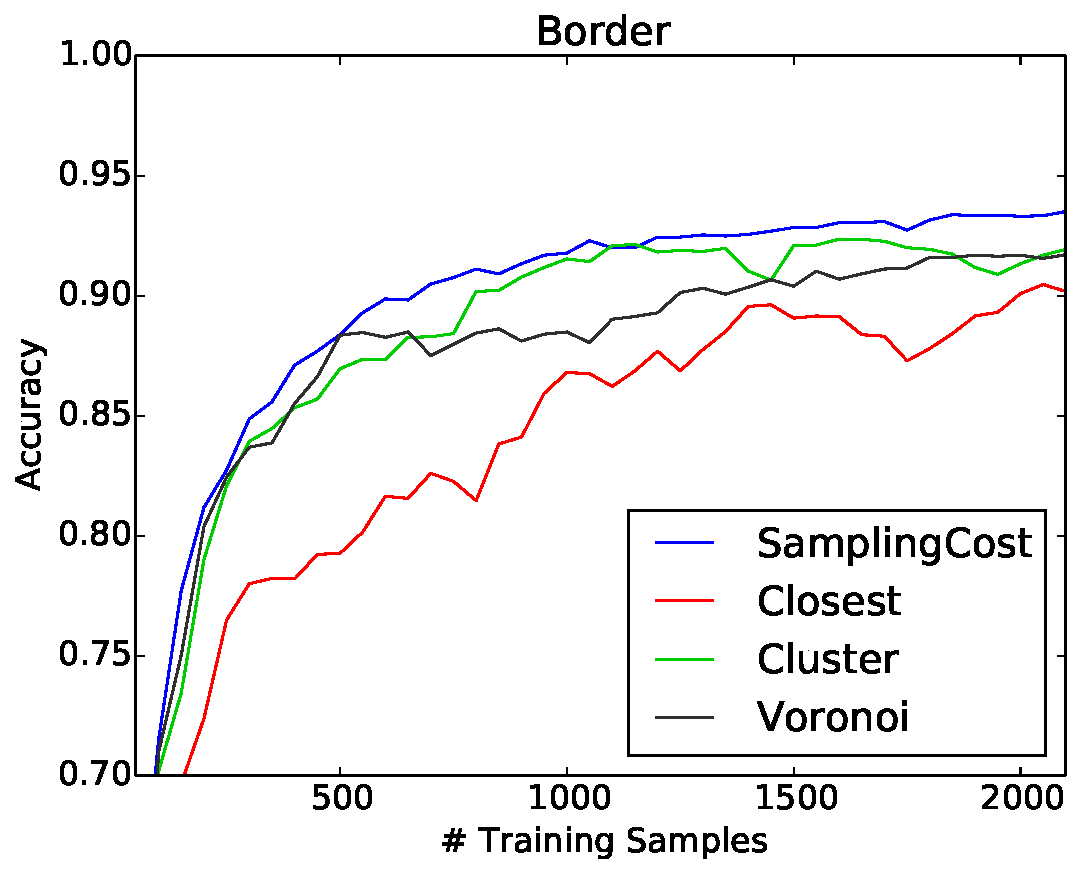
\includegraphics[width=0.24\textwidth]{Images/Toy/Border_random_07_accuracy.pdf}}
	\subfloat{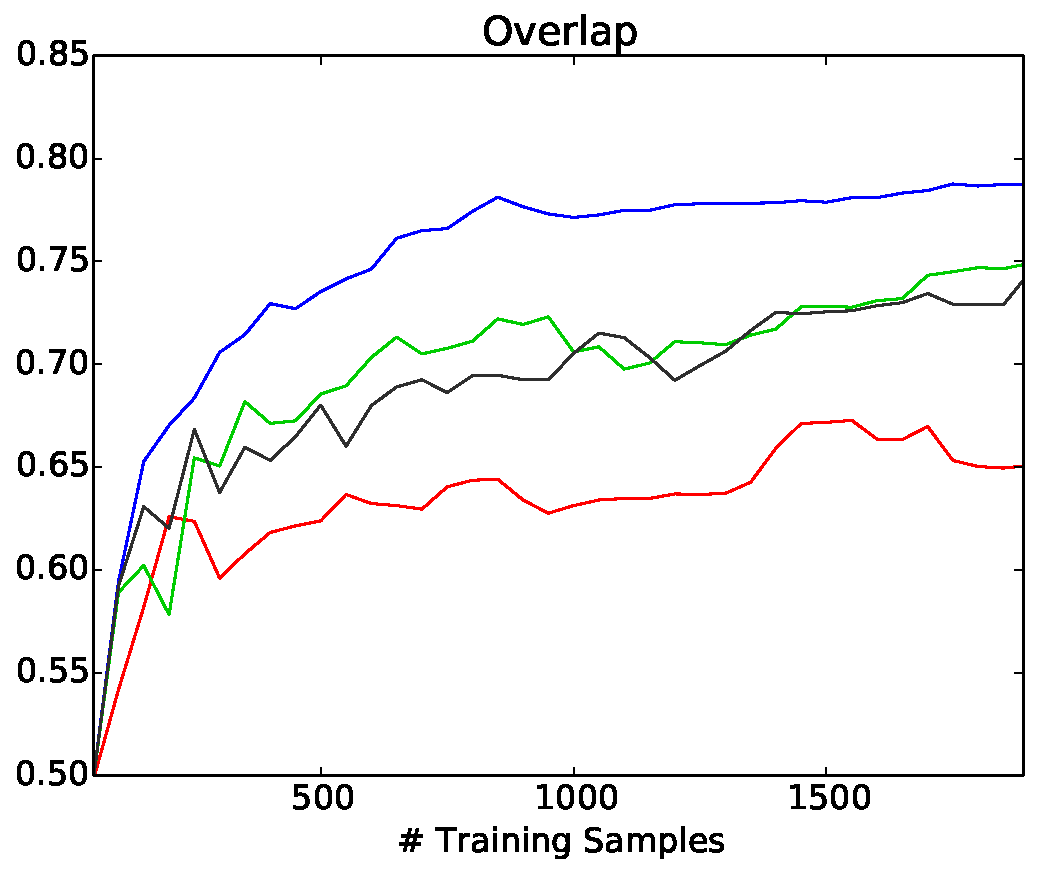
\includegraphics[width=0.23\textwidth]{Images/Toy/Overlap_random_07_accuracy.pdf}}
        \caption{Accuracies in the course of training for the artificial data sets. 
        \textit{SamplingCost} leads continuously and especially performs on the \textit{Overlap} data set better than the rest.}
        \label{fig:Toy1Graphs}
\end{figure}
\textit{Closest} quickly loses touch, whereas \textit{SamplingCost} is in the lead throughout training. 
 
\section{Application Setup}
In our scenario, an autonomous robot is exploring a garden environment (Fig. 4\ref{outdoorScenario}) in a random scheme.
\begin{figure}
\centering
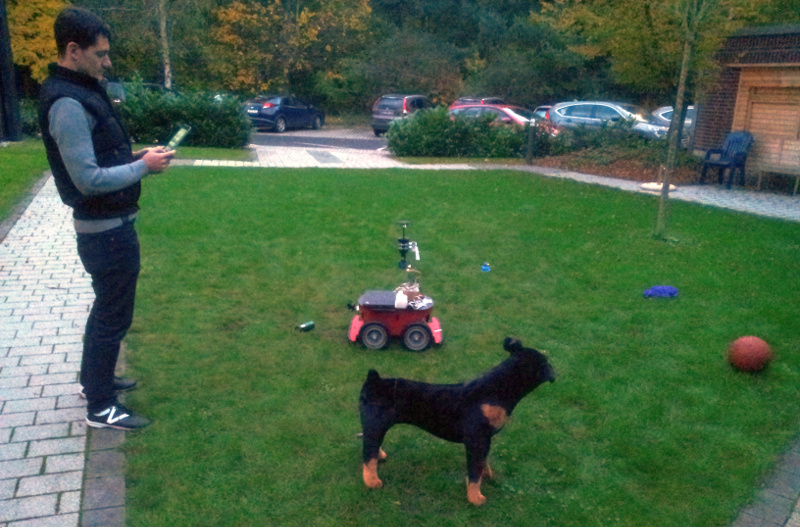
\includegraphics[width=0.35\textwidth]{Images/General/Scenario.jpg}
\caption{Typical scene of the interactive scenario. The robot drives randomly on the grass area and encounters various objects. The 
user follows the image-stream on the iPad and can label approached objects.}
\label{outdoorScenario}
\end{figure}
The user interacts in real-time with the robot by labeling approached objects via an iPad. 
Labeled objects are incrementally incorporated into the model and learned immediately enabling a direct reaction of the system.
New objects can be introduced at any time.\\
Whenever an object is approached, the robot stops in front of it within a certain distance. If the user does not provide a label, the robot announces the recognized class.
Unknown objects as well as uncertain classifications are expressed explicitly. 
Object specific actions are only executed in case of confident classifications. Actions may include oral comments as well as driving behaviors such as 
avoiding or driving over. Objects are always avoided whenever they are classified as unknown or uncertain. 
Since the garden border is treated as any other object, but coupled strictly with avoidance, the robot stays within the grass area.\\
We used the Pioneer platform of Adept Mobile\-Robots with a front-mounted Playstation Eye camera, which is directed on the 
ground and captures the scene with a frame rate of 120 $Hz$.
Computation is done by a Lenovo ThinkPad, also mounted on the robot.
A color-based grass segmentation algorithm detects obstacles whenever their representation
deviates significantly from an environment model. Since this model is adapted dynamically, a high range of color variety can be handled.

\subsection{Filtering}
The distance between near objects and the robot is used for the situation recognition. 
Far distanced objects should be ignored because an approach of these is uncertain. If an object is too close, a reaction, for example an avoiding maneuver, should be performed. 
Hence, only objects within a certain distance-window are relevant for learning. We mapped this window on image regions, 
as it can be seen in Figure \ref{attentionField}.
\begin{figure}
\centering
\subfloat{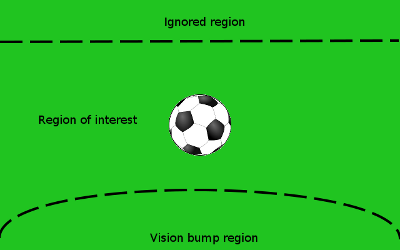
\includegraphics[width=0.25\textwidth]{Images/General/VisualField.png}}~
\subfloat{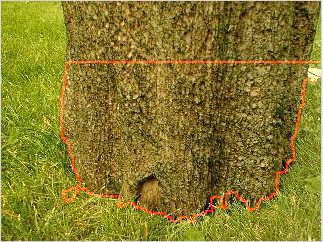
\includegraphics[width=0.209\textwidth]{Images/General/TallObject.jpg}}
\caption{Left: Partition of the input image. Objects are only examined as long as they are in the region of interest. Overlaps with the vision
bump region end the examination and trigger a reaction. Information within the top marked area is ignored completely.
Right:
Masked area (red) of a close tree stump. The upper part of the image is disregarded even though it belongs to the object.
}
\label{attentionField}
\end{figure}
The upper part is ignored for processing, based on the assumption that far objects are located there. 
Close objects can be found on the bottom part of the image. Therefore, the robot stops as soon as the object contours overlap this lower part.
However, the first assumption fails sometimes, for example concerning nearby tall objects as depicted in Figure \ref{attentionField} on the right.
In this case available object information is thrown away. \\
Whenever multiple objects are segmented, only the dominant object is regarded. Dominance exists if one object is pixel-wise at least two times larger than the rest.
In case of similar sized objects the learning is deactivated, but the collision avoidance is still performed.
As long as an object is within the region of interest, object information is collected. Information is processed further only if the so-called 
vision bump region gets overlapped by the object. 
Therefore, only directly approached objects are considered, and the ones which are just passed by are ignored. 
Depending on whether a user-label was provided, either learning or classification follows the vision bump.

\subsection{Apps}\label{labelingapp}
All data, for example trained images, classes and class-actions, are stored on the laptop. Apps act as clients and access data temporarily using a WIFI connection. The Labeling-app allows the user to manage previously recorded images. Object classes can be edited as well as corresponding actions. 
The robot pauses whenever this app is executed preventing any inconsistency between app and laptop on one hand and unsupervised
robot actions on the other.\\
The Streaming-App provides insight into the current robot state during execution. Images as well as segmentation contours are streamed and can be accessed here. 
Whenever an object is approached, the user has the opportunity to label it for a certain time.
Thereby the current classification result as well as its confidence are displayed to facilitate the decision whether to label the current sequence or not.
Labeling leads to an immediate, incremental learning process using the actual sequence as training data.
Otherwise the sequence gets classified and possibly related actions are performed. 

\subsection{Data Representation}
\begin{wrapfigure}{}{0 pt}
\centering
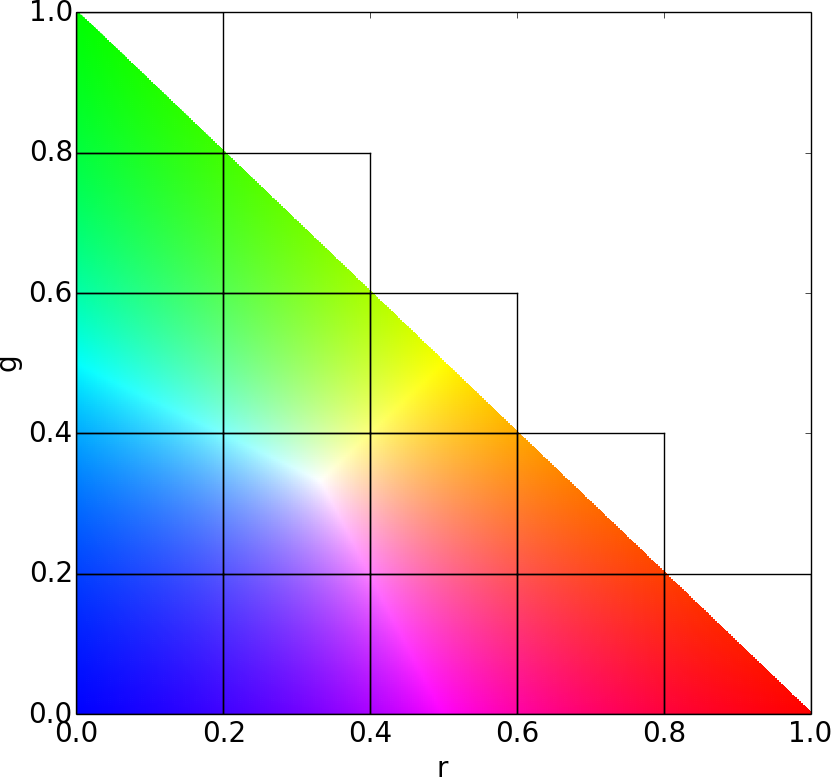
\includegraphics[width=0.18\textwidth]{Images/General/RgChromacityQuads.png}
\caption{Histogram binning of the rg-chromaticity space.}
\label{rgTable}
\end{wrapfigure}
Since visual objects in our application scenario
are mostly non-textured, we chose a rg-chromaticity color histogram as feature representation instead of local features such as SIFT \cite{Lowe:1999:ORL:850924.851523}. 
Especially for outdoor scenarios, it is important to encode the color of an object independently from prevalent illumination.
One step in this direction is to use an intensity invariant color space such as rg-chromaticity \cite{Jain:2005:HFR:1062383}
which represents one color by the normalized proportions of red, green and blue instead of using their intensities (as done in the RGB space).
The normalization removes intensity information and enables a two dimensional representation.
Figure \ref{rgTable} visualizes the employed binning for six intervals resulting in a 21-dimensional feature vector. 
In addition, we normalize the feature vector to a total sum of 1 to achieve size invariance. 

\subsection{Sequence Confidence}\label{classification}
We employ a confidence estimation to identify unknown objects and perform object specific action only for highly confident classifications.
Fischer et al.\ analyzed recently various geometric certainty measures for LVQ \cite{2673548}. Their accuracy vs.\ rejection results 
were comparable to those of statistical models. One of them, called Relative Similarity is particularly attractive since it is 
already normalized. However, this measure defines a measure for one input sample whereas we are interested in the estimation of whole sequences. Therefore we
extended the measure in the following way.
Let $\Gamma= \{\mathbf{x}_i\}_{i=1}^s$ be the set of features belonging to one sequence with the length $s$. The confidence that this sequence belongs to class $\beta$ is defined as
\begin{equation*} 
C(\Gamma)_\beta = \frac{1}{s}\sum_{i=1}^sc(\mathbf{x}_i)_\beta,
\end{equation*}
where $c(\mathbf{x}_i)_\beta$ is the confidence that feature $\mathbf{x}_i$ belongs to $\beta$.
The classification of a sequence can be inhomogeneous. 
Since the Relative Similarity provides only a confidence for the nearest class, we use the following definition if 
$\beta$ is not the nearest class:
\begin{equation*}
c(\mathbf{x},\beta) = \frac{d_1(\mathbf{x}) - d_2(\mathbf{x},\beta)}{d_1(\mathbf{x})+d_2(\mathbf{x},\beta)}
\end{equation*}
$d_1(\mathbf{x})$ denotes the distance to the closest prototype, while $d_2(\mathbf{x},\beta)$ is the distance to the closest prototype of class $\beta$.
The sequence-confidence $C(\Gamma)_\beta$ varies between $[-1...1]$.\\
Two thresholds $\theta_{u}$ and $\theta_{c}$ assign a certainty category $\Omega$ to a given sequence confidence C
\begin{equation*} 
\Omega(C) = \begin{cases}C < \theta_{u} & $unknown object$ \\ C >= \theta_{u} $ and $C< \theta_{c} & $uncertain classification$ \\ else & $confident classification$ \end{cases}
\end{equation*}

\section{Interactive Scenario Evaluation}
We recorded a data set consisting of 40 Objects during the interactive scenario in an outdoor garden environment.
Green colors were avoided to simplify the task for the color-based grass segmentation. 
Objects were approached five times in sunny and five times in cloudy conditions. The approaches were conducted from different directions. 
Each of them contains the last ten images before the vision bump was triggered. 
Altogether 4000 images were recorded. \\
Figure \ref{fig:outdoorRuns} depicts examples for sequences containing objects with similar
pose in different weather conditions. 
\begin{figure}
        \centering
        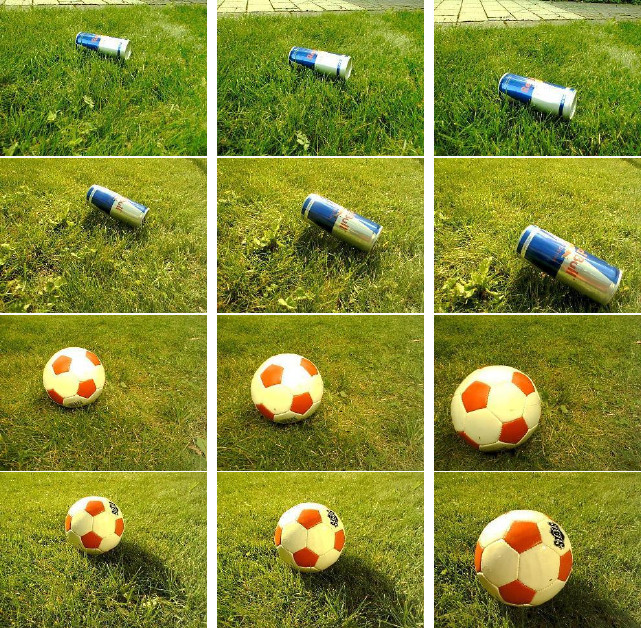
\includegraphics[width=0.3\textwidth]{Images/Outdoor/Runs.jpg}
        \caption{Objects approached in different lighting conditions. 
        Each row shows the first, fifth and tenth image of one approach. 
        The upper row of each object was recorded in cloudy and the bottom row in sunny conditions.}
        \label{fig:outdoorRuns}        
\end{figure}
Usually, objects are only increasing in size and therefore the variance within one sequence is small.
Figure \ref{fig:outdoorCases} illustrates additional challenges comprised by this data set.
\begin{figure}
        \centering
	\vspace{1 pt}
	\subfloat[]{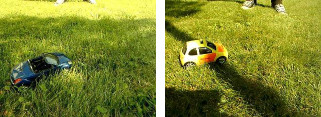
\includegraphics[width=0.2\textwidth]{Images/Outdoor/Cases/Cases_a.jpg}
	\label{fig:outdoorCasesA}
	}
	\vspace{1 pt}        
	\subfloat[]{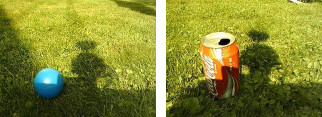
\includegraphics[width=0.2\textwidth]{Images/Outdoor/Cases/Cases_b.jpg}
	\label{fig:outdoorCasesB}
	}
	\vspace{1 pt}
	\subfloat[]{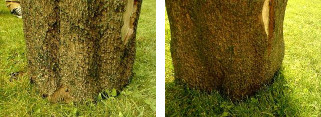
\includegraphics[width=0.2\textwidth]{Images/Outdoor/Cases/Cases_c.jpg}
	\label{fig:outdoorCasesC}
	}\vspace{1 pt}
	\subfloat[]{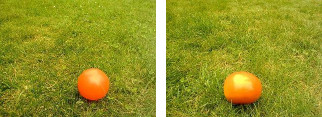
\includegraphics[width=0.2\textwidth]{Images/Outdoor/Cases/Cases_d.jpg}
	\label{fig:outdoorCasesD}
	}
	\vspace{1 pt}
	\subfloat[]{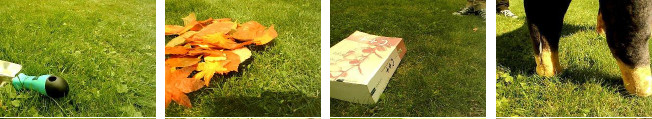
\includegraphics[width=0.405\textwidth]{Images/Outdoor/Cases/Cases_e.jpg}
	\label{fig:outdoorCasesE}
	}        
	\vspace{1 pt}
	\subfloat[]{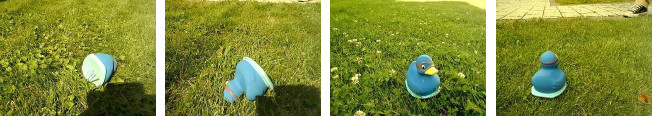
\includegraphics[width=0.405\textwidth]{Images/Outdoor/Cases/Cases_f.jpg}
	\label{fig:outdoorCasesF}
	}        
        \caption{Challenges of the Outdoor data set. Objects covered in various degrees by shadows cast by environmental obstacles 
        such as trees or buildings (a) or by the robot itself (b). Sunlight and auto-exposure cause a darker object representation (c). Specular highlights (d). 
        Occlusions by the image border (e). Various object poses (f).}
        \label{fig:outdoorCases}        
\end{figure}
Objects were completely or partly covered by hard or soft shadows (Fig.~\ref{fig:outdoorCasesA}). 
When the sun was in the back of the robot, a self-shadow was cast in driving direction and covered objects nearby (Fig.~\ref{fig:outdoorCasesB}). 
In the case of approaching the sun, objects were especially dark because of self-shadowing and auto exposure control (Fig.~\ref{fig:outdoorCasesC}).
Direct spotlighting caused various sized specular highlights (Fig.~\ref{fig:outdoorCasesD}). 
Occlusions were mainly caused by the image border (Fig.~\ref{fig:outdoorCasesE}) and some tall objects always exceeded the image height when being approached.
Arbitrary pose variations (Fig.~\ref{fig:outdoorCasesF}) were generated by throwing objects from a low height on the ground. 
Unfortunately, the mentioned cases do have a certain impact on the feature vector. Figure \ref{fig:featureImpacts} illustrates this by
visualizing outputs of all relevant processing steps - namely segmentation, color space transformation and histogram binning.
\begin{figure}
        \centering
        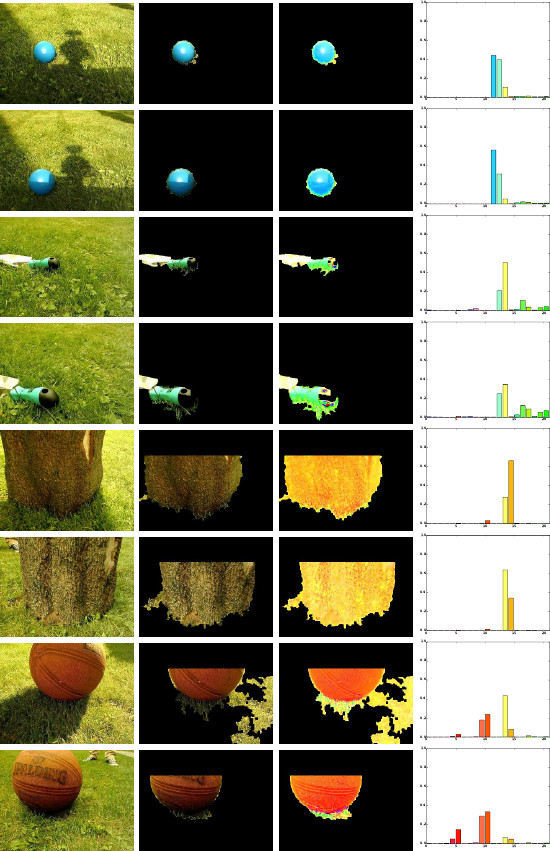
\includegraphics[width=0.4\textwidth]{Images/Outdoor/Impacts.jpg}
        \caption{Impacts of various challenges on the results of relevant processing steps. 
        Each row depicts from left to right the recorded picture,
        the segmented object, the appearance in rg-chromaticity space and the color histogram. Illustrated are the effects of shadows (blue ball), occlusions (shovel), direct sunlight (stump) 
        and wrong segmentations (basketball).}
        \label{fig:featureImpacts}
\end{figure}
The blue ball example depicts the influence of robot-cast shadows. Both pictures are taken from the same approach.
Note that the shadowed region is still visible in the rg-chromaticity space even though
it is slightly less distinct. This leads to a shift towards the dark blue bin and changes the representation.
The shovel below illustrates the effect of occlusion. Its front part exceeds the image border in the course of an approach and removes a chunk of yellow portion 
from the representation. The stump shows another influence caused by lighting conditions. Its self-shaded appearance is clearly 
more brown than the yellow illuminated version below. All colors are shifted towards yellow due to the sunlight. Particularly grayscales such as the silver shovel or 
its black handle are mapped to the same yellow bin. 
Therefore, this dimension is the most prominent within the data set. 
The histogram difference for the basketball example is caused by improper segmentation, which occurred in a few cases. Since a bigger region is segmented,
the brown bins for the real object color are proportionately smaller due to normalization. The opposite case, in which not the entire object is segmented, also happened, but is similar to 
the occlusion example.\\
\subsection{Results}
When it comes to online learning, the assumption of data being i.i.d. \cite{Carlevarino00anincremental} often does not apply.
In our interactive scenario, various consecutive images of the same object are recorded in constant pose and more or less constant lighting conditions. 
If the user decides to label this object sequence, all belonging samples are trained in the recorded order. In case of classification, the whole sequence is unknown
for the classifier. Therefore, it is important to analyze the generalization to new object
sequences, since this is the practically relevant case. 
It is particularly interesting considering the given small variance within one sequence compared to the high variance across different sequences. 
Hence, we trained the learning architecture sequence-wise in chunks of ten images. However, the order of the sequences was random.
Table \ref{tab:OutdoorChunkWise} shows the results for seven training sequences per object, achieved by each placement strategy. 
Also depicted is the outcome for training in random order with $70\%$ of the data. 
\begin{table}
\centering
\caption{Results for the Outdoor data set with sequenced and random ordered training.}
\label{tab:OutdoorChunkWise}
\begin{tabular}{c|ccc}
\textit{Sequence-order} & Test acc. & Train acc. & Nodes\\\hline
\rule{0pt}{10pt}
SamplingCost & \textbf{61.38} & 91.04& 232.0\\
Closest & 59.58 & 88.04 & 245.8\\
Cluster & 59.18 & 88.96 & 235.6\\
Voronoi & 58.81 & 89.22 & \textbf{231.3}
\end{tabular}
\par\vspace{5 pt}
\begin{tabular}{c|ccc}
\textit{Random-order} & Test acc. & Train acc. & Nodes\\\hline
\rule{0pt}{10pt}
SamplingCost & \textbf{81.58} & 85.94 &\textbf{234.8}\\
Closest & 78.03 & 83.23 & 253.4\\
Cluster & 78.55 & 83.06 & 247.0\\
Voronoi & 81.18 & 85.62 & 236.6
\end{tabular}
\end{table}
The heavy performance decline on the test set for the sequence-wise order is striking. This allows the conclusion that generalization to completely unseen sequences is more challenging.
Consequently, the chosen feature representation is not robust enough against the different variations contained in the data set. 
A lot of directly illuminated objects share a similar representation with a big concentration on the yellow bin and the variance
of the representation across different objects is often smaller than those of the same object across different approaches.
Nevertheless, a high accuracy is achieved 
when images are shuffled randomly. Even though a high variance is given for the data set, the difference of images within one sequence is usually small. 
As soon as one image of each sequence is contained in the training set, the major part of variance is covered and high rates are possible. \\
The nets are also larger for the sequence-wise order, which means that more errors occurred during training. One cause is the dependence of the GLVQ-updates 
on a random order since the cost-function has to be minimized in a stochastic gradient descent scheme. But the main reason is that, during
training, the generalization from sequence to sequence is limited too. Therefore, whenever a new sequence is trained, the classifier makes more mistakes until prototypes are added.\\
\textit{SamplingCost} achieves the best results, but compared to the artificial data sets, the performance difference between placement strategies is rather small.
The image data set contains many times more classes but less samples per class. Therefore, the choice among these samples is more limited per class, which leaves
little leeway to choose good or bad candidates. Furthermore, the data in the high dimensional space is not broadly distributed but rather strongly clustered. 
Hence, the already limited choice makes additionally not a big difference.
\begin{wrapfigure}{}{0 pt}
\centering
	\subfloat{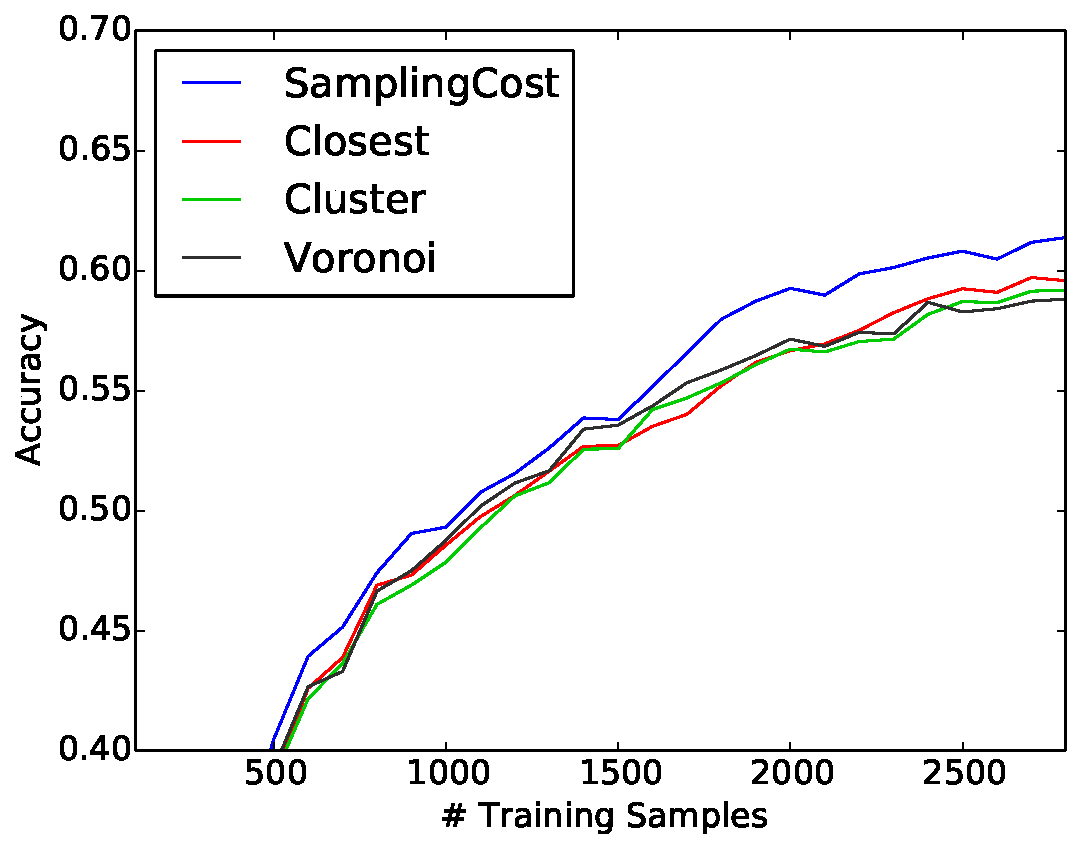
\includegraphics[width=0.23\textwidth]{Images/Outdoor/OutdoorEasy_chunksRandomEqualCountPerLabel_07_accuracy.pdf}	}                
        \caption{Test-accuracies for sequence-wise training on the Outdoor data set.}
        \label{fig:OutdoorChunkWise}
\end{wrapfigure}
Figure \ref{fig:OutdoorChunkWise} illustrates accuracies during training.
All placing strategies perform similar but \textit{SamplingCost} leads continuously throughout the training.
Figure \ref{fig:OutdoorHist} depicts the prototype distributions among all classes. 
\begin{figure}
        \centering
        \vspace{0 pt}
	\subfloat{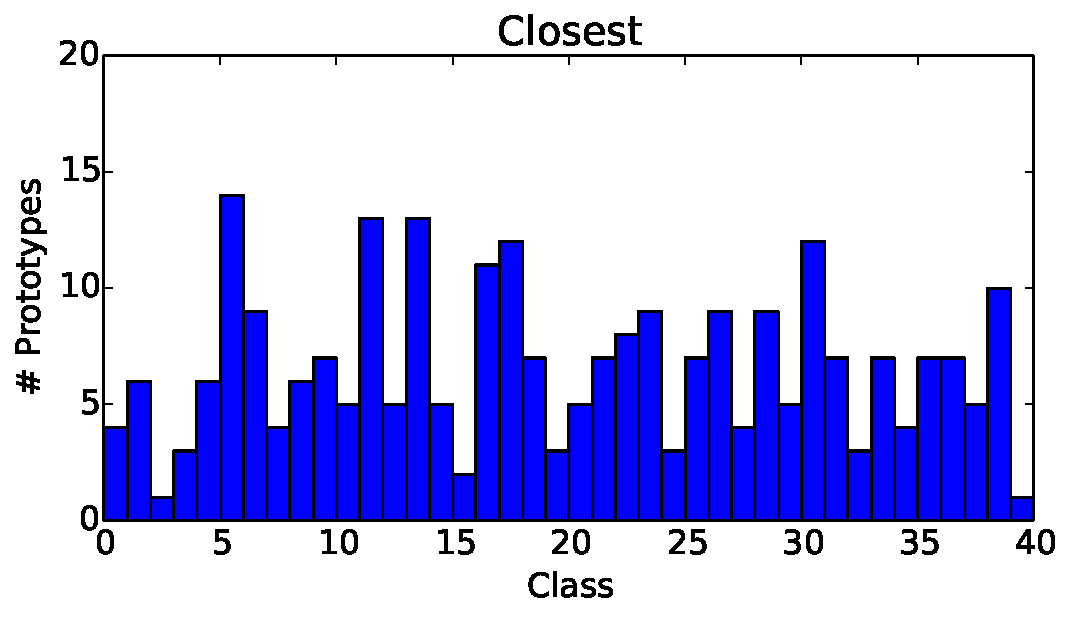
\includegraphics[width=0.23\textwidth]{Images/Outdoor/OutdoorEasy_chunksRandomEqualCountPerLabel_07_Closest_hist.pdf}}
	\vspace{0 pt}
	\subfloat{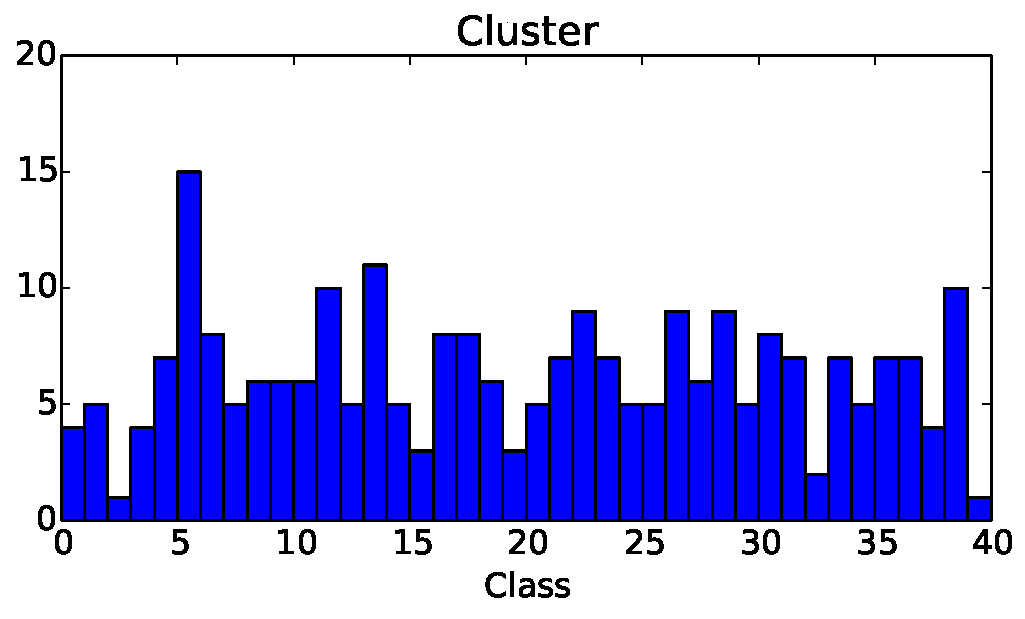
\includegraphics[width=0.23\textwidth]{Images/Outdoor/OutdoorEasy_chunksRandomEqualCountPerLabel_07_Cluster_hist.pdf}}        
        \vspace{0 pt}
	\subfloat{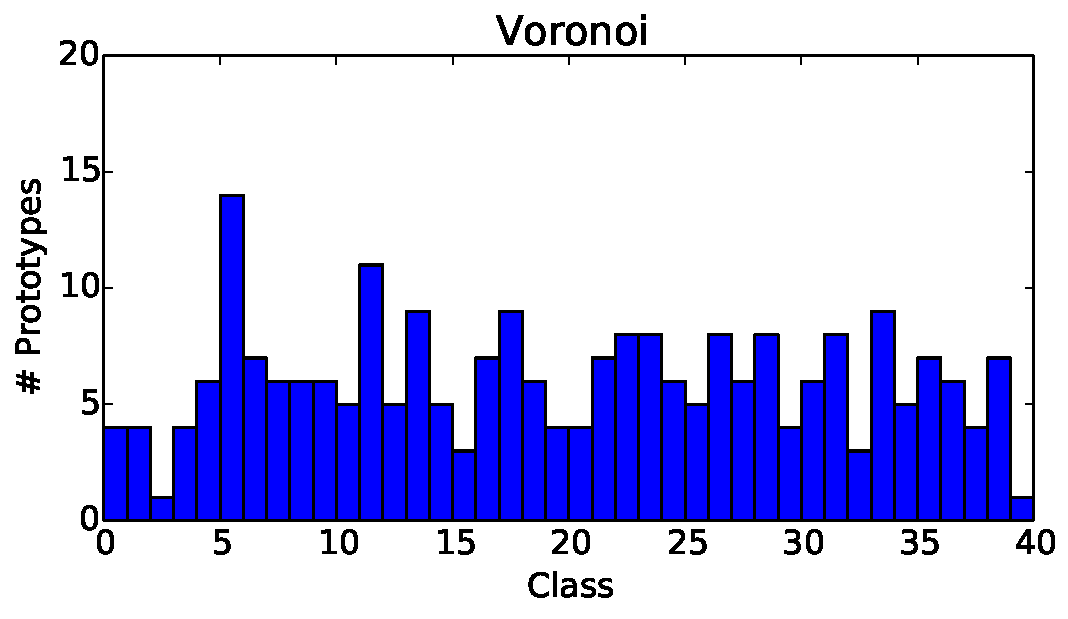
\includegraphics[width=0.23\textwidth]{Images/Outdoor/OutdoorEasy_chunksRandomEqualCountPerLabel_07_Voronoi_hist.pdf}}        
	\vspace{0 pt}
	\subfloat{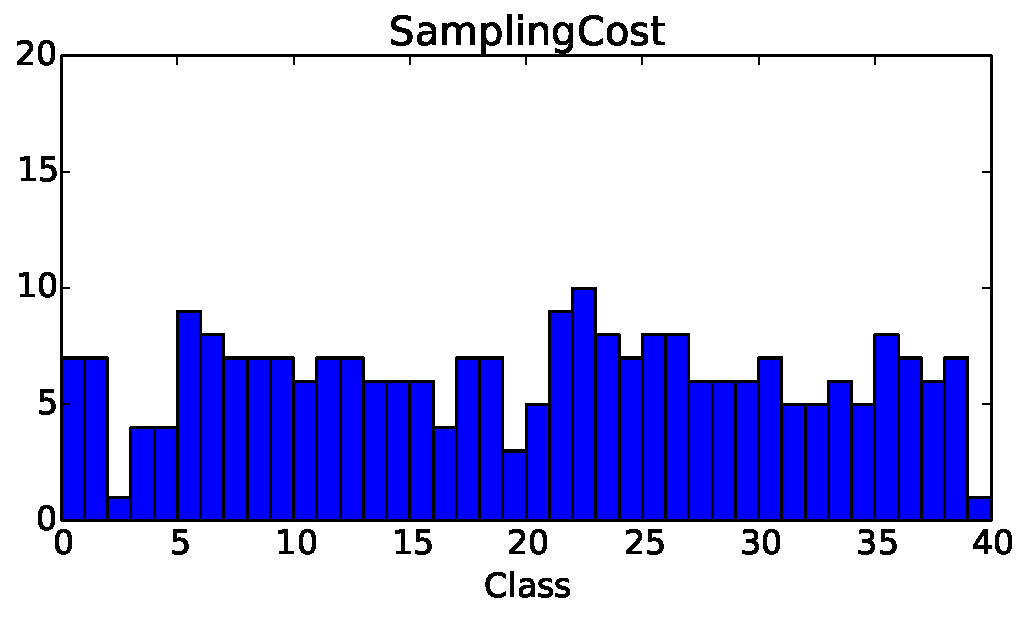
\includegraphics[width=0.23\textwidth]{Images/Outdoor/OutdoorEasy_chunksRandomEqualCountPerLabel_07_SamplingCost_hist.pdf}}        	
        \caption{Prototype distributions for the Outdoor data set.}.
        \label{fig:OutdoorHist}
\end{figure}
The fact that \textit{Closest} shows an irregular distribution with several difficult objects claiming more than ten prototypes,
suggests that it provides too many prototypes for certain classes. 
\textit{SamplingCost} distributes nodes very evenly since the cost-function optimization encourages regular spreading as already seen in the 
experiments with artificial data.\\
Table \ref{tab:OutdoorHardest} ranks the top four objects claiming most prototypes and therefore being hardest to discriminate by \textit{SamplingCost}. 
\begin{table}
\centering
\caption{The four objects receiving the most prototypes by \textit{SamplingCost}. 
The column on the right shows the classes which were the most often confused with the object.}
\def \imageWidth{0.09\textwidth}
\label{tab:OutdoorHardest}
\begin{tabular}{ c | l }
    Object & Mostly confused with \\ \hline
    %&&&\\
      \\\vspace{1 pt}
      \subfloat{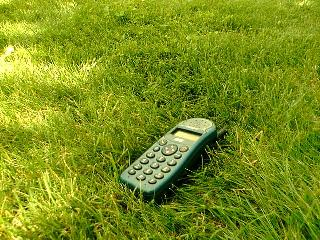
\includegraphics[width=\imageWidth]{Images/Outdoor/Ranked/Hard/Philips_1_10.jpg}} 
    & \subfloat{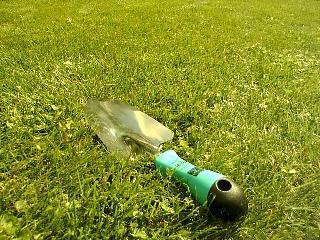
\includegraphics[width=\imageWidth]{Images/Outdoor/Ranked/Hard/Confused/Paddle_3_10.jpg}}~
      \subfloat{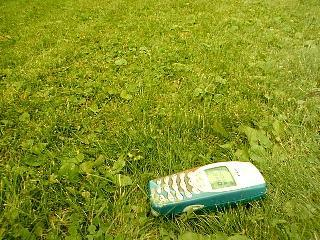
\includegraphics[width=\imageWidth]{Images/Outdoor/Ranked/Hard/Confused/Nokia_8_10.jpg}}~
      \subfloat{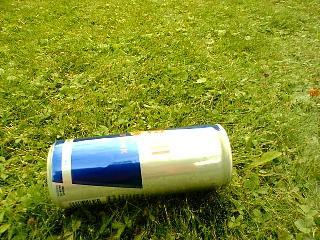
\includegraphics[width=\imageWidth]{Images/Outdoor/Ranked/Hard/Confused/RedBull_7_10.jpg}}
      \\\vspace{1 pt}
      \subfloat{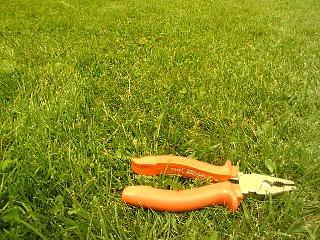
\includegraphics[width=\imageWidth]{Images/Outdoor/Ranked/Hard/Forceps_7_10.jpg}} 
    & \subfloat{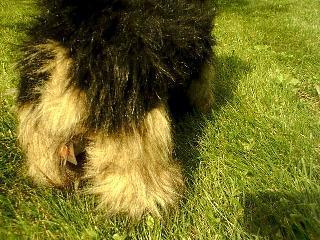
\includegraphics[width=\imageWidth]{Images/Outdoor/Ranked/Hard/Confused/SmallDog_4_10.jpg}}~
      \subfloat{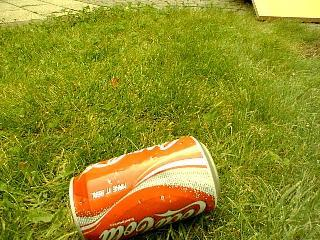
\includegraphics[width=\imageWidth]{Images/Outdoor/Ranked/Hard/Confused/Coke_9_10.jpg}}~
      \subfloat{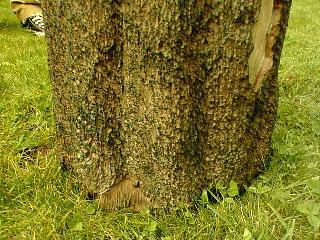
\includegraphics[width=\imageWidth]{Images/Outdoor/Ranked/Hard/Confused/Stump_3_10.jpg}}
      \\\vspace{1 pt}
      \subfloat{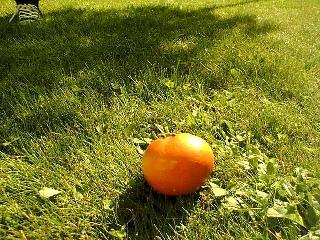
\includegraphics[width=\imageWidth]{Images/Outdoor/Ranked/Hard/Tomato_1_10.jpg}} 
    & \subfloat{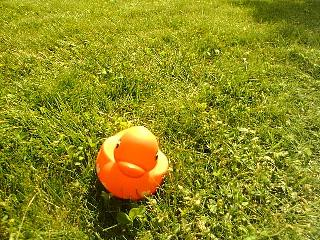
\includegraphics[width=\imageWidth]{Images/Outdoor/Ranked/Hard/Confused/RedDuck_3_10.jpg}}~
      \subfloat{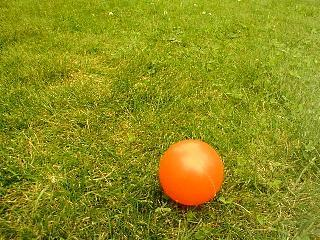
\includegraphics[width=\imageWidth]{Images/Outdoor/Ranked/Hard/Confused/RedBall_3_10.jpg}}
      \\\vspace{1 pt}
      \subfloat{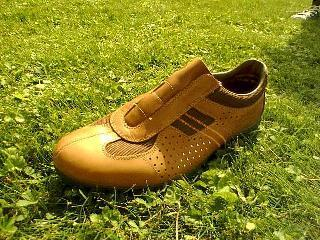
\includegraphics[width=\imageWidth]{Images/Outdoor/Ranked/Hard/Shoe_1_10.jpg}} 
    & \subfloat{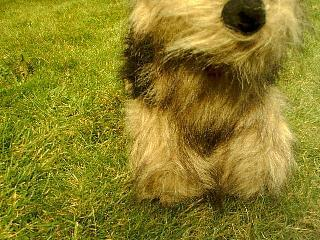
\includegraphics[width=\imageWidth]{Images/Outdoor/Ranked/Hard/Confused/SmallDog_6_10.jpg}}~
      \subfloat{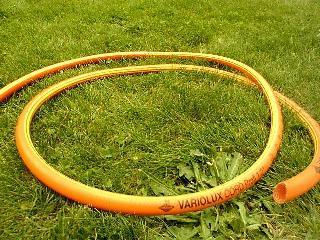
\includegraphics[width=\imageWidth]{Images/Outdoor/Ranked/Hard/Confused/Tube_1_10.jpg}}~
      \subfloat{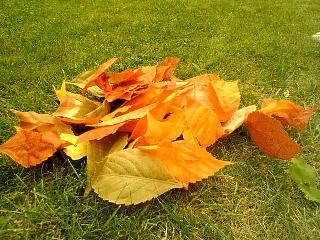
\includegraphics[width=\imageWidth]{Images/Outdoor/Ranked/Hard/Confused/Leaves_7_10.jpg}}

    \end{tabular}
\end{table}
Most confusions are reasonable but the cause for mistaking the red pliers for the brown-black plush toy or the brown stump seems to be unclear 
because of their actual different color representation. 
However, a closer examination reveals that the major part of the actual red pliers, 
especially the front metal part, is yellow or orange in sunny conditions. This is also true for the two other objects as illustrated in Figure \ref{fig:ConfusionsOutdoor}.\\
\begin{figure}
        \centering
        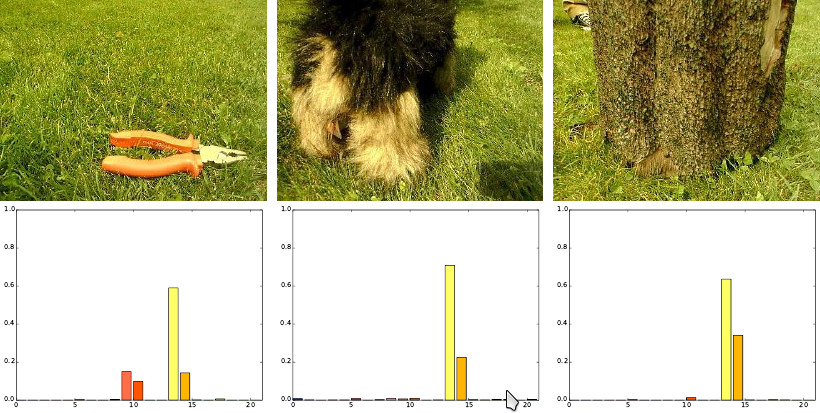
\includegraphics[width=0.3\textwidth]{Images/Outdoor/Confusions.jpg}
        \caption{Similarity due to the sunlight. Actually different colored objects are shifted to the same representation by direct sunlight.}
        \label{fig:ConfusionsOutdoor}        
\end{figure}
Objects claiming the fewest prototypes by all placement algorithms are shown in Figure \ref{fig:OutdoorEasy}. 
\begin{figure}
        \centering
        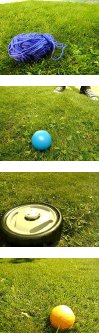
\includegraphics[width=0.48\textwidth]{Images/Outdoor/Easy.jpg}
        \caption{Easiest classes within the Outdoor data set. The wool was the only object requiring just one prototype across all algorithms. }
        \label{fig:OutdoorEasy}
\end{figure}
The wool requires exclusively a single node since it is the only purple object. The remaining easy objects were covered by 3-5 prototypes
depending on the placement strategy. A rare color distribution paired 
with view angle independence are the key properties for effortless discrimination.

\paragraph{Comparison with Incremental SVM}
To get a better picture of the performance of the online learning system in combination with the proposed \textit{SamplingCost} insertion strategy, 
a comparison with the incremental support vector machine (iSVM), discussed in \cite{cauwenbergs01incrementaldecremental}, \cite{Diehl03svmincremental} and \cite{Laskov:2006:ISV:1248547.1248616}, was done. 
We used the iSVM implementation provided by Diehl\footnote[1]{Code at \url{https://github.com/diehl/Incremental-SVM-Learning-in-MATLAB}} \cite{Diehl03svmincremental} with Gaussian kernel ($C=1024$, $\sigma=0.05$). 
The iSVM stores the support vectors, and additionally a set of  reserve vectors which are the points that can be seen at one time. 
Since this is the counterpart to our window of recent samples $\Phi$, we limited its
size to $200$ entries. The iSVM was trained in a one-vs-all scheme.
We increased considerably the prototype insertion frequency to achieve  maximum performance. 
So far we coupled the insertion strategy with GLVQ. Here we also analyze the performance in combination with the 
generalized matrix LVQ (GMLVQ) \cite{Schneider:2009:ARM:1737743.1737754}. This classifier is more powerful since it incorporates metric learning
 of the input space.\\
Apart from our Outdoor data set we also evaluated the well-known benchmark COIL-100 \cite{CAVE_0189}  with the same feature 
representation. This RGB-image data set consists of 72 views for 100 objects each. 
These are placed in the coordinate origin and rotated around the Z axis in steps of  $5\,^{\circ}$.
Image size is $128 \times 128$ pixel. 
As in \cite{conf/iccv/WallravenCG03} a subset of 17 views per object, resulting in views every $20\,^{\circ}$, are used for training.\\
Table \ref{tab:OutdoorSVM} shows the accuracy as well as the stored number of prototypes / support vectors after an increasing number of training examples.
\captionsetup{position=top}
\begin{table}
\centering
\caption{Comparison to the incremental SVM on the Outdoor and COIL data set. \textit{SamplingCost-GMLVQ} learns additionally the metric of the input space. 
Pairs of test-accuracy and nodes which are not pareto dominated are marked in bold. }
\subfloat[Outdoor-Sequenced]{
\begin{tabular}{c|ccc}
\textit{} & \shortstack{Acc. / Nodes  \\500 samples} & \shortstack{Acc. / Nodes  \\1500 samples} & \shortstack{Acc. / Nodes  \\2800 samples} \\\hline
\rule{0pt}{10pt}
SamplingCost-GLVQ & 42.9 / 116.4 & 58.6 / 446.2& 64.3 / 948.8\\
SamplingCost-GMLVQ & \textbf{44.1 / 100.4} & \textbf{59.3 / 376.6} & \textbf{67.1 / 773.5}\\
iSVM & 40.6 / 363.3 & 57.5 / 777.0 & 65.2 / 1347\\
\end{tabular}
}
\par\vspace{5 pt}
\subfloat[COIL-100]{

\begin{tabular}{c|ccc}
\textit{} & \shortstack{Acc. / Nodes  \\500 samples}  & \shortstack{Acc. / Nodes  \\1000 samples}  & \shortstack{Acc. / Nodes  \\1700 samples}  \\\hline
\rule{0pt}{10pt}
SamplingCost-GLVQ & 83.5 / 337.8 & 90.4 / 560.0  & 93.6 / 810.0\\
SamplingCost-GMLVQ & \textbf{85.0 / 330.6} & \textbf{91.9 / 539.5}& \textbf{94.7 / 760.0}\\
iSVM & 85.6 / 1834  & 92.7 / 2139 & \textbf{95.6 / 2501}\\
\end{tabular}
}
\label{tab:OutdoorSVM}
\end{table}
Our algorithm performs better than iSVM on the Outdoor data set and uses thereby a less complex model. The combination with the GMLVQ has always 
a higher accuracy and less nodes compared to the GLVQ one. Regarding the COIL data set, iSVM has a slightly higher accuracy but requires  a considerably
more complex model. Additionally the complexity, i.e.\ number of support vectors
generated by iSVM, cannot be limited unlike for incremental LVQ variants.

\section{Conclusion}
Our incremental learning architecture combines GLVQ with a placement strategy optimizing the cost-function on the basis of a limited sample history.
The comparison on artificial and image based data sets showed the superiority of the proposed placement strategy over current heuristic-based strategies.
The optimization can be done efficiently with linear complexity and enables the handling of overlapping distributions. 
Paired with the GMLVQ, our architecture achieves better results than the incremental SVM in most cases and requires thereby a clearly less complex model.\\
We demonstrated the architecture within an interactive online learning scenario on a mobile robot. Objects, lying outdoor on the lawn, are trained in real-time 
and are instantly incorporated into the model representation, enabling a direct reaction of the system.
The used rg-chromaticity color histogram turned out to be insufficiently robust to deal with changes due to
various lighting conditions. Generalization to completely unseen image sequences, as necessary for the scenario, is therefore only partially possible. 
However, the representation is not coupled to our learning architecture and can be easily exchanged.
\newpage

% trigger a \newpage just before the given reference
% number - used to balance the columns on the last page
% adjust value as needed - may need to be readjusted if
% the document is modified later
%\IEEEtriggeratref{8}
% The "triggered" command can be changed if desired:
%\IEEEtriggercmd{\enlargethispage{-5in}}

% references section

% can use a bibliography generated by BibTeX as a .bbl file
% BibTeX documentation can be easily obtained at:
% http://www.ctan.org/tex-archive/biblio/bibtex/contrib/doc/
% The IEEEtran BibTeX style support page is at:
% http://www.michaelshell.org/tex/ieeetran/bibtex/
%\bibliographystyle{IEEEtran}
% argument is your BibTeX string definitions and bibliography database(s)
%\bibliography{IEEEabrv,../bib/paper}
%
% <OR> manually copy in the resultant .bbl file
% set second argument of \begin to the number of references
% (used to reserve space for the reference number labels box)
\bibliographystyle{IEEEtran}
\bibliography{IEEEabrv,OnlineLearningIJCNN}

% that's all folks
\end{document}

\iffalse
ToDo:

subfloats labeling Benni fragen
Test-Accuracy in Captions